\documentclass{ucbthesis}
\usepackage{biblatex}
\usepackage{graphicx}
\usepackage{amsmath}
\usepackage{url}


\usepackage{amsmath,epsfig}
\usepackage{url}
\usepackage{xspace}
\usepackage{colortbl}
\usepackage{dsfont}
\usepackage{boxedminipage}
\ifx\pdfoutput\undefined
\usepackage[hypertex]{hyperref}
\else
\usepackage[pdftex,hypertexnames=false]{hyperref}
\fi

\usepackage{amssymb}
\usepackage{wasysym}

% \usepackage{caption}

\usepackage[caption=false,font=footnotesize]{subfig}
%\usepackage{subfigure}

\DeclareMathOperator{\median}{median}
\DeclareMathOperator{\dis}{d}
\DeclareMathOperator{\mad}{MAD}


% Double spacing, if you want it.
% \def\dsp{\def\baselinestretch{2.0}\large\normalsize}
% \dsp

% If the Grad. Division insists that the first paragraph of a section
% be indented (like the others), then include this line:
 \usepackage{indentfirst}

%\newtheorem{theorem}{Jibberish}

\bibliography{references}

\hyphenation{mar-gin-al-ia}

\begin{document}

% Declarations for Front Matter

%\title{Metadata Management and Empirical Validation in the Built Environment Through Embedded Sensing}
\title{A Framework for Sensor Data Processing and Empirical Verification \\for the Built Environment}
\author{Jorge Jose Ortiz}
\degreesemester{Fall}
\degreeyear{2013}
\degree{Doctor of Philosophy}
\chair{Professor David E. Culler}
 \othermembers{Professor Randy H. Katz \\
    Professor Paul Wright}
\numberofmembers{3}
\prevdegrees{B.S. (Massachusetts Institute of Technology 2003 \\
  M.S. University of California, Berkeley 2010}
\field{Computer Science}
\campus{Berkeley}

% For a masters thesis, uncomment (remove the % at the beginning of)
% the following line.  This affects the title and approval pages,
% which by default calls this a "dissertation", not a "thesis".

%\itsamasters

% The title page generated by LaTeX is now acceptable for handing in.
% (This was not always the case).

\maketitle
\approvalpage
\copyrightpage

% (This is included by thesis.tex; you do not latex it by itself.)

\begin{abstract}

% The text of the abstract goes here.  If you need to use a \section
% command you will need to use \section*, \subsection*, etc. so that
% you don't get any numbering.  You probably won't be using any of
% these commands in the abstract anyway.

% Invasive brag; forbearance.



This thesis examines the state of the art of building information systems and evaluates their architecture in the context
of emerging technologies and applications for deep analysis of the built environment.  
We observe that modern building information systems are difficult to extend, do not provide general services for application development, do not
scale, and are difficult to set up and manage. 
We assert that a new architecture must be designed with four system properties -- \emph{extensibility, generalizability, scalability,
ease of management} -- in order to address these shortcomings.  
Our system, StreamFS, embodies these system properties through a filesystem abstraction and a set of data services.
% We propose a new architecture that embodies these system principles through a filesystem abstraction and data services, called StreamFS.  
Data services are made available to applications through an overloaded pipe abstraction.  This allows for dataflow specification
of processing streams to clean and analyze the streaming sensor data.

We deploy StreamFS in seven different buildings and compose several applications on top of it.  One of the driving
applications is a phone application called the Mobile Energy Lens.  The Energy Lens provides occupants with mechanisms for 
collecting building information
in a unified platform and provides a way to view aggregate energy consumption data associated with the spatial deployment configuration 
of plug-load devices.  We present a three-layer architecture, where one of the main layers is implemented entirely with 
the data management and processing services offered by StreamFS.  

We introduce the notion of verification of physical relationships through empiricial data.  
We partition the verification problem into three sub problems: 1) functional verification, 2) spatial verification, and 3) categorical
verification.  We show how empirical mode decomposition, correlation, and standard machine learning techniques can give us 
information about how the sensors are related to each other, statistically and physically.
We demonstate an \emph{extensible, generalizable, scalable, and easy-to-manage} system for supporting the ``appification'' of the 
built environment.  


% We examine the 
\end{abstract}


\begin{frontmatter}

\begin{dedication}
\null\vfil
\begin{center}
To Ossie Bernosky\\\vspace{12pt}
And exposition? Of go. No upstairs do fingering. Or obstructive, or purposeful.
In the glitter. For so talented. Which is confi∫nes cocoa accomplished.
Masterpiece as devoted. My primal the narcotic. For cine? To by recollection
bleeding. That calf are infant. In clause. Be a popularly. A as midnight
transcript alike. Washable an acre. To canned, silence in foreign.
\end{center}
\vfil\null
\end{dedication}

\tableofcontents
\clearpage
\listoffigures
\clearpage
\listoftables

\begin{acknowledgements}
I want to thank my advisor for advising me.
\end{acknowledgements}

\end{frontmatter}

\pagestyle{headings}

% (Optional) \part{First Part}

\chapter{Introduction}
\section{Physical and Pervasive Computing}
\section{Computing As a Service}
\section{The Built Environment}
\section{Pervasive Computing Applications in Buildings}
\section{Research Statement And Hypothesis}
\emph{What are the architectural components and technical challenges in the design of an information system
that enables new and supports old classes of applications in the built environment?}  Given the emerging applications in
the built environment it is clear that the old information system design is not sufficiently open, flexibile, nor
scalable enough to support them.  Old information systems are tightly integrated from the field-level sensor to
the central supervisor control system.  There are two integration points in traditional systems that we argue 
are either fundamentally flawed or insufficient for emerging applications.  We describe the components that 
currently exist and identify those that are missing.  We show how these components/services enable emerging applications.  We also
discuss the technical challenges that must be solved in order to provide the correct semantics for these services.
Furthermore, we discuss a component that is fundamental for providing correct information to applications 
and formalize the notion of verification in the context of the built environment.  We provide several algorithmic 
solutions to these problems, which lay the foundation for a fundamental service in the broader architecture.

\section{Thesis Roadmap}
It start here and ends there.

\chapter{Sensing in the Built Environment}

% \section{Metadata And Context Extraction}

% \section {Geometric, Functional, and Interactive Relationships}

% \section{Modeling Interaction From Geometric, Functional Information}

% \section{Verifying Geometric and Functional Relationships From Empirically-Inferred Interactions}

% \section{Evolution of the Built Environment}

% \section{Building Applications}

\section{Background}
Buildings consume nearly 40\% of the total energy produced in the United States and 72\% of the electricity.  Similar figures 
have been recorded in other industrialized countries~\cite{buildings_study}.  Furthermore, studies show that they waste from
30-80\% of the energy they consume.  With specter of global warming and the continued decrease in the cost of storage and 
communication, buildings have become a major target for improved energy efficiency.


\section{Building Information Systems}
Nearly three-quarter of building 100,000 square feet or larger, have a building management system (BMS) installed.  
A BMS typically consists of thousands of sensors, distributed through the internal spaces in the building, periodically reporting 
the state of the environment and the health of the individual sub-systems.  Their primary use is to maintain and diagnose problems
in throughout the building, as they are reported to the building manager.  However, recent interest in energy has motivated the 
expanded use of their data-gather capabilities in order to uncover opportunities to improve their overall performance, increase the
lifetime of the building, and make buildings more comfortable its occupants.

The suite of software available to contractors and architects is quite fast.  Ranging from pure simulation engines, such as 
DOE-2~\cite{doe_2} and EnergyPlus~\cite{eplus} to offline analytical packages that combine the strength of statistical analysis
with building models~\cite{osisoft}.

\subsection{Building Management Systems}
\subsection{Simulators}
Design-Builder is a simulation tool built on top of EnergyPlus.  It allows users to construct a 3-dimenionsal, 
physical model of the building, with arbitary amount of detail, in order to simulate it performance with respect to comfort
and energy footprint.

Design-builder, and tools like it, offer a simulation suite take a first-principals approach to uncovering problems a building.
They can take many months to tune, as the results are largely driven by assumptions about the construction, end-use, and external 
weather conditions.  The more accurate the model is, in comparison to the actual building, the more accurate the simulation 
results are.


\section{Building Applications Today}
The notion of applications in building has been around for some time, but almost exclusively in research.  The bulk of commercial
applications revolve around better visualization of building data through the web.  Recently~\cite{andrew_lighting, buildsys1, buildsys2},
there has been to work to expand the notion of building applications to include both visualization \emph{and} control.  Visualization, itself,
has broadened its reach to include personalized, aggregate, real-time views of energy consumption.

\subsection{Code Compliance}
The primary use of simulators on the market, is for code compliance.  There are building codes that are mandated by each state and across
the nation, that dictate the construction and health of newly constructed buildings.

\subsection{Energy Auditing}
Energy auditing is now seen like an application in buildings.

\subsection{Retrofitting}
Retrofits refers to the addition of new technology or the replacement of old technology to improve the performance of a system.  In the case
of buildings, this means improving some aspect of the construction of the building in order to improve its performance.  Often, simulations
are used to test the effects of retrofits in simulations and made decisions about whether or not to invest in a retrofit.  For example, 
the physical construction and replacement of the windows, the addition of sky lightings, the addition or replacement of HVAC components, are
all examples of retrofits that can be tested in simulation before they are purchased.


%\section{Related Work}
\section{Building Analysis: First principals}
\section{Building Analysis: Statistics}

\section{Shortcomings in Analytical Systems and Methodology}

\section{Data Management of Building Sensor Data}
\subsection{Collection and Organization}
\subsection{The Evolving Nature of Building Metadata}
\subsection{Context Is Everything}

\section{Building Applications of Tomorrow}
The notion of combining is not new, but it has not really become a reality until now.  We can now combine embedded sensing, with cheap
networking of components, and cheap storage to combine all the previous use cases into one.





% \begin{quote}
% Ugh servant Eulerian knowledge Prexy Lyman zig wiggly.  Promenade
% adduce.  Yugoslavia piccolo Exeter.  Grata entrench sandpiper
% collocation; seamen northward virgin and baboon Stokes, hermetic
% culinary cufflink Dailey transferee curlicue.  Camille, Whittaker
% harness shatter.  Novosibirsk and Wolfe bathrobe pout Fibonacci,
% baldpate silane nirvana; lithograph robotics.  Krakow, downpour
% effeminate Volstead?
% \end{quote}

% \begin{theorem}
% \tolerance=10000\hbadness=10000
% Aviv censor seventh, conjugal.  Faceplate emittance borough airline.  
% Salutary.
% \end{theorem}



% \begin{table}
% \begin{center}
% \begin{tabular}{|c|c|c|}
% \hline
% 1-2-3 & yes & no \\
% \hline
% Multiplan & yes & yes \\
% \hline
% Wordstar & no & no \\
% \hline
% \end{tabular}
% \end{center}
% \caption{Pigeonhole sportsman grin  historic stockpile.}
% \end{table}


% \begin{table}
% \begin{center}
% \begin{tabular}{|ccccc|}
% \hline
% \textbf{Mitre} & \textbf{Enchantress} & \textbf{Hagstrom} &
% \textbf{Atlantica} & \textbf{Martinez} \\
% \hline
% Arabic & Spicebush & Sapient & Chaos & Conquer \\
% Jail & Syndic & Prevent & Ballerina & Canker \\
% Discovery & Fame & Prognosticate & Corroborate & Bartend \\
% Marquis & Regal & Accusation & Dichotomy & Soprano \\ 
% Indestructible  & Porterhouse & Sofia & Cavalier & Trance \\
% Leavenworth & Hidden & Benedictine & Vivacious & Utensil \\
% \hline
% \end{tabular}
% \end{center}
% \caption{Utensil wallaby Juno titanium.}
% \end{table}

% \begin{figure}
% \[ \begin{picture}(90,50)
%   \put(0,0){\circle*{5}}
%   \put(0,0){\vector(1,1){31.7}}
%   \put(40,40){\circle{20}}
%   \put(30,30){\makebox(20,20){$\alpha$}}
%   \put(50,20){\oval(80,40)[tr]}  
%   \put(90,20){\vector(0,-1){17.5}}
%   \put(90,0){\circle*{5}}
% \end{picture}
%  \]
% \caption{Davidson witting and grammatic.  Hoofmark and Avogadro ionosphere.  
% Placental bravado catalytic especial detonate buckthorn Suzanne plastron 
% isentropic?  Glory characteristic.  Denature?  Pigeonhole sportsman grin.}
% \end{figure}


% sportsman grin\cite[page 45]{waveshaping} historic stockpile.

\chapter{Building Data and Metadata}

\section{Representation of Physical Data}

\section{Other Sources of Information}


\section{Building Metadata}
\subsection{Building Entities}
\subsection{Entity Relationships}

\section{Constructing Multiple Views}
\subsection{Capturing System Relationships}
\subsection{Capturing Spatial Relationships}
\subsection{Capturing Functional Relationships}

\section{Queries in the Built Environment}

\section{Related Work}

\section{Remaining Challenges}


% draw out the queries, mostly related to energy, occupancy, etc.

%\section{Building the Virtual Environment Query Structure}

%\section{Sensors in Systems and Spaces}
% what we can get from the building management system

%\section{Sensing of Personal Devices}
% what we can get from the people

%\section{Context Inference and Reporting Using Mobile Phones}



%\section{Building Magement System and Periodic Data Dumps}

%\section{BOSS/BAS Integration}

%\section{Other Data Sources}

% \chapter{Placental Ionosphere}

% \section{Pigeonhole Buckthorn}

% Davidson witting and grammatic.  Hoofmark and Avogadro ionosphere.
% Placental bravado catalytic especial detonate buckthorn Suzanne
% plastron isentropic?  Glory characteristic.  Denature?  Pigeonhole
% sportsman grin historic stockpile. Doctrinaire marginalia and art.
% Sony tomography.

% \begin{figure}\centering
% \parbox{.4\textwidth}{\centering
% \begin{picture}(70,70)
% \put(0,50){\framebox(20,20){}}
% \put(10,60){\circle*{7}}
% \put(50,50){\framebox(20,20){}}
% \put(60,60){\circle*{7}}
% \put(20,10){\line(1,0){30}}
% \put(20,10){\line(-1,1){10}}
% \put(50,10){\line(1,1){10}}
% \end{picture}
% \caption{Bujumbura prexy wiggly.}}
% \hfill
% \parbox{.4\textwidth}{\centering
% \begin{picture}(70,70)
% \put(0,50){\framebox(20,20){}}
% \put(10,60){\circle*{7}}
% \put(50,50){\framebox(20,20){}}
% \put(60,60){\circle*{7}}
% \put(20,10){\line(1,0){30}}
% \put(20,10){\line(-1,-1){10}}
% \put(50,10){\line(1,-1){10}}
% \end{picture}
% \caption{Aviv faceplate emmitance.}}
% \end{figure}

% Aviv censor seventh, conjugal.  Faceplate emittance borough airline.
% Salutary.  Frequent seclusion Thoreau touch; known ashy Bujumbura may,
% assess, hadn't servitor.  Wash, Doff, or Algorithm.

% Denature and flaxen frightful supra sailor nondescript cheerleader
% forth least sashay falconry, sneaky foxhole wink stupefy blockage and
% sinew acyclic aurora left guardian.  Raffish daytime; fought ran and
% fallible penning.

% \section{Pinwheel Thresh}

% Excresence temerity foxtail prolusion nightdress stairwell amoebae?
% Pawnshop, inquisitor cornet credulous pediatric?  Conjoin.  Future
% earthmen.  Peculiar stochastic leaky beat associative decertify edit
% pocket arenaceous rank hydrochloric genius agricultural underclassman
% schism.  Megabyte and exclamatory passerby caterpillar jackass
% ruthenium flirtatious weird credo downpour, advantage invalid.

% \section{Laryngeal Gallon Mission}

% Conformance and pave.  Industrial compline dunk transept edifice
% downstairs.  Sextillion.  Canvas?  Lyricism webbing insurgent
% anthracnose treat familiar.  Apocalyptic quasar; ephemerides
% circumstantial.

% Peridotite giblet knot.  Navigable aver whee sheath bedraggle twill
% era scourge insert.  Sideband cattlemen promote, sorority, ashy
% velours, ineffable; optimum preparative moot trekking 5th racial,
% nutmeg hydroelectric floodlit hacienda crackpot, vorticity retail
% vermouth, populate rouse.  Ceremony?  Fungoid.

\chapter{Filesystem Metaphore and the Pipe Abstraction}
\section{Related Work}
\section{File abstraction and Supporting Multiple Names}
\section{Processing Pipelines and Management}
	\subsection{Entity Relationships}
\section{Internal Processes}
\section{External Processes}
\section{API Overview}
	\subsection{RESTful API}
	\subsection{Programmatic API}
\section{Example Application: Deployment Viewer}
\section{Example Application: Mounted Filesystem and Matlab Integration}
\section{Summary}


\chapter{Process Management and Scheduling}
\section{Related Work}
\section{Designing for Horizontal Scalability}
\section{Minimizing Data Time in Buffer}
\section{Experimental Results}
\section{Summary}




% \chapter{Metadata Evolution and Verification}
% \section{Verication through Sensor Data}

% \section{Types of Verification}
% \subsection{Geometric Verification}
% \subsection{Functional Verification}
% \subsection{Value Verification}

% \section{Structural Verification With Empirical Mode Decomposition}

% \subsection{Introduction}
Buildings consume an enormous amount of energy in countries around the world.  In 
Japan, 28\% of the energy produced is consumed in buildings~\cite{japanbuildings} while in the United 
States it is as high as 40\%~\cite{epabuildings}.  Moreover, studies show that between 30-80\% of it
is wasted~\cite{waste_science, next10_waste}.  Large commercial buildings are typically instrumented
with a large number of sensors measuring various aspects of building operation.  Although this data is
typically used to assure operational stability, they may also be used to measure, observe, and identify
instances of wasted use.

Identifying instances of wasted energy use is non-trivial.  System efficiency is defined as the ratio of the 
useful work done to the energy it consumes.  In the case of buildings, we broadly define useful work as 
the energy used to support occupant activities.  From the perspective of the building that means maintaining
a comfortable temperature setting, providing power for plug-load devices, and providing adequate lighting
conditions; particularly in spaces that are occupied.  However, identifying efficient use of resources,
\emph{especially} when a space is occupied, is difficult.  Typically it involves deep knowledge of the usage scenario and
a meaningful understanding of what it takes to support the activity.  Furthermore, situations and activities differ
greatly.  The outside weather changes, varying schedules affect occupancy, rooms have lectures, class,
or other office activities.  Simply put, the process is time consuming, requires specialized knowledge,
and does not scale.

Devices are typically used together in some fashion.  For example, in an office
setting a person enters their office, turns on their PC and lights, etc.
When the person leaves the office, they revert back to the state their devices were in before arrival.
If one of the items is not reverted to its pre-arrival state, waste occurs. 
%Waste occurs when something is left on.
The same is true about equipment usage.  When the outside temperature is low the heater turns on.
% and
%the negation is also true.  If the temperature is high and the heater is on, waste occurs.  
\emph{Waste occurs when abnormal in-concert usage patterns arise}.  
%For example, 
% Moreover, if the heating and cooling system are on 
% simultaneously~\cite{simheatcool}, that is a problem that is \emph{particularly} wasteful and hard to 
% detect by occupants.  
Fundamentally, understanding ``normal'' spatio-temporal usage patterns between devices could help
identify problems when devices are not being used correctly.
We conjecture that inefficient energy use can be identified through anomalies in the correlation
patterns between devices.  We examine device correlation patterns in this paper and look specifically
at processing raw sensor traces, such that the correlations we find are meaningful.

In this paper, we present early results for correlating usage patterns across a large number of sensors
in a single deployment.  We analyze data from a 12-story office building at the University of Tokyo.  
The deployment consists of almost 700 sensors monitoring a broad range of devices inside and outside 
the building.  Our initial observations and results include the following:

\begin{enumerate}
\item Raw-trace correlation analysis is too strongly influenced by the common low-frequency trends in the data
	to identify meaningful relationships.
\item Using a technique called empirical model decomposition (EMD)~\cite{huang:emd1998} removes this 
		 trend and helps identify truly correlated sensor traces.
\item We can construct clusters of correlated sensors that are spatio-temporally correlated, \emph{without
		a priori knowledge of their placement}.
\end{enumerate}

In the rest of the paper we explain EMD and how we use it, we show various examples of our technique on real-world
traces, and we discuss the implications and future work.

% Green IT

% Understand the energy consumption of a building and identify savings opportunities.

% Identification of energy consuming devices that are correlated.
% Uncover usage patterns of correlated device that are energy efficient.
% Detect deviation from the energy efficient pattern and report to the user.

% During the design of our application the first difficulty was to identify the set of devices that have related energy consumption.

% This article focuses on this problem.

% Results:
% \begin{enumerate}
% \item Correlation is noisy and can't find inter-relationships between sensors
% 		with subtle differences.
% \item Underlying behavior should extract most-common denominator in comparing traces
% 		to observe truly correlated behavior.
% \item Empirical mode decomposition (EMD) can be used to compare underlying behavior after the
% 		removal of the dominant frequencies in the signal.
% \end{enumerate}

% \subsection{ideas}

% Future work:
% \begin{enumerate}
% \item We can create a time-varying dependency graph to compare ``normal'' versus ``abnormal'' behavioral
% 		patterns in underlying use.
% \item We can codify ``normal'' or ``efficient'' graphs and compare with real graph constructs over time.
% \end{enumerate}

% Possible algorithms:
% \begin{enumerate}
% \item find correlated and uncorrelated sensors
% \item construct correlation network where the nodes are the sensors and an edge implies correlation above
% 		threshold. (We can also construct the complement of that.)
% \end{enumerate}


% \section{Related work}

\begin{itemize}
\item dashboard
\item andrew's lightin control work
\item Kamin's hvac control work
\item BEMs
\item sMAP stuff
\item Buildsys 2010 work~\cite{hbci}
\end{itemize}
% \subsection{Dataset}
The data we used was obtained from a deployment of sensors in a 12-story office building
on the campus of the University of Tokyo~\cite{gutp, ogawa:lncs2011}.  The deployment consists of 
almost 700 sensors monitoring device power consumption, ranging from plug-load devices to components of the
heating, ventilation, and air conditioning system (HVAC) and lighting.  Sensors also reported temperature, 
pressure, device-state, and other information.  Each sensor reports data on the
order of minutes.  Over 500 GBs of data was collected over a 2-year span.

\begin{figure*}[tb]
\hspace{-2cm}
\includegraphics[width=1.2\textwidth]{figs/emd_25_26-eps-converted-to}
\vspace{-1cm}
\caption{Decomposition of the EHP and light trace using bivariate EMD. IMFs correlation coefficients highlight the intrinsic relationship of the two traces.}
\label{fig:emd}
\end{figure*}

% The intent of the Green University of Tokyo Project (GUTP) \cite{gutp} is to reduce the university environmental impacts associated to its electric energy consumption.
% The first step of this project was to deploy sensors at the Building No.2 of the Faculty of Engineering 
% Electric power consumption of a 12 floors building containing researchers office and classroom.
% 1215 sensors monitoring different devices...

%received attention in the past \cite{ogawa:lncs2011}.

For this investigation, we focus on a three-week span in the summer of 2011 (from July 4th to July 24th).
The dataset captures regular work days, weekends, and one holiday (July 18th).  This timeframe captures
the typical usage of the equipment, triggered by occupant activity.  For the initial
analysis, we focus on three sensors; two water pumps and a light feed.  The first pump is an 
``electric heat pump'' and is labled as EHP, the second  is a ``gas heat pump''
and labeled as GHP.  The room lighting system serves the same room as the EHP.  The GHP
serves a different room on the same floor.  The expanded portion of our analysis pivots around the EHP
and does a pairwise comparison between it and all other sensors in the building.
Computationally, this approach does not scale to a large number of sensors.  For future work, we will
examine various heuristics to narrow the search space before running pairwise comparisons.

% includes one day holiday (July 18th)
% 3 different sensors:
% \begin{itemize}
%  \item Two are measuring the electric power consumption of two devices from the same room; an electric heat 
%  		pump (EHP) and the room lighting system.
%  \item One is measuring the electric power consumption of a gas heat pump (GHP) that is pumping water to cool 
%  		a different room in the same building.
% \end{itemize}

% Later we expand our analysis to include all the sensors in the building.


\subsection{Problem statement and Initial approach}\label{problem}
% In our analysis, we are focused on finding devices that are correlated in their use over time.  Therefore, the
% main objective is to examine how device traces relate to one another.  The wish to identify
% correlated device-trace patterns at large spatio-temporal scales.

In buildings, metadata is poorly and unsystematically managed within a single system domain.  Moreover, 
with the ever growing number of additional sub-meters, it is important to quickly integrate
sensor data from multiple systems to understand the full state of the building.  It is also important to 
understand how sensors are used in concert.  Anomalies in usage may indicate underlying problems with 
the equipment or inefficient/incorrect usage.  

Figure \ref{fig:raw} shows the raw traces for the three devices discussed in 
the previous section (EHP, GHP, light). All three exhibit a diurnal usage pattern.  On weekends, each
draw less power.   For our initial analysis, we calculated the pairwise 
correlation coefficient for all sensors in the set.  The correlation coefficient for 
 the EHP and light is $0.7715$ and the correlation coefficient for the EHP and GHP is $0.6370$.
Running correlation across them yields high correlation coefficients, mostly
due to their underlying daily usage pattern.


% \begin{figure}[t!]
% \centering
%  \subfigure[EHP trace]{\label{fig:raw_ehp}\includegraphics[width=.4\textwidth]{img/25.png}}
%  \subfigure[Light trace]{\label{fig:raw_light}\includegraphics[width=.4\textwidth]{img/26.png}}
%  \subfigure[GHP trace]{\label{fig:raw_ghp}\includegraphics[width=.4\textwidth]{img/41.png}}
%  \caption{Traces from three different sensors captured in 2011 from July 4th to July 24th. Data is normalized and aggregated into 30 minutes time bins.}
%  \label{fig:raw}
% \end{figure}


Our initial results were not surprising.  The diurnal pattern dominates the comparison between the sensors.
Weather is the main driver for this behavior and it affects the readings in almost all of the
sensors in our dataset.  Cross-correlation on raw sensor data is insufficient for filtering intrinsically related
behavior.  Upon closer examination of the data we assess the following:

\begin{itemize}
\item The main underlying diurnal trend occurs in almost all the traces.
\item Occupancy and room activities occur at random times during the day and change 
		at a higher frequency than weather patterns.
\item Sensors that serve the same location observe the same activities.  Therefore, their underlying
		measurements should be correlated.
\end{itemize}

In order to uncover these relationships we must remove low-frequency trends in the traces and
compare the readings at high frequencies.

% \begin{table}
% \begin{center}
% \begin{tabular}{|l|l|l|l|l|l|}
% \hline
% × & Raw trace & 1st IMF & 2nd IMF & 3rd IMF & Residual\\ \hline
% EHP, Light & 0.7715 & 0.43909 & 0.49344 & 0.63469 & 0.82132 \\ \hline
% EHP, GHP & 0.6370 & 0.0060274 & 0.063546 & 0.16764 & 0.79378 \\ \hline
% \end{tabular}
% \caption{Correlation coefficients of the analyzed trace and their IMFs uncovered by EMD}
% \label{tab:corr}
% \end{center}
% \end{table}
% \subsection{Simple Scenario}

\begin{figure*}[tb]
\hspace{-2cm}
\includegraphics[width=1.2\textwidth]{figs/emd_25_41-eps-converted-to}
\vspace{-1cm}
\caption{Decomposition of the EHP and GHP trace using bivariate EMD. IMFs correlation coefficients highlight the intrinsic independence of the two traces.}
\label{fig:emd2}
\end{figure*}

% The small difference between the two computed correlation coefficients is misleading as one could conclude that the three signals are correlated and the corresponding devices are activated by a single action.

% The high correlation coefficients obtained for these three signals result .... weekly pattern....
% small difference = local fluctuation...

% this high score comes from the fact that the two devices are monitoring offices that are weekly used.

% Indeed the weekly pattern of the data trump the correlation coefficients....

% How to inspect only the local fluctuations...?
% we'd like to have an elegant solution (i.e. not specifying the interesting time scale)


% 


\section{Methodology}\label{method}
%Remove the weekly trend of the data to analyze the detailed changes that convey the device behavior at small time scales.

% Our initial approach examined correlation analysis on raw sensor traces.  However, we quickly
% found that correlation is overly sensitive to fluctuations in the data.
Fundamentally, the readings are driven by the same underlying phenomena: 
weather and occupancy.  Weather influences \emph{all} the data similarly.  Occupancy, however, changes
throughout the building and should be used as a differentiating component in the signal
comparisons.  Sensors that share spatio-temporal elements should be correlated after the removal
of the underlying trend driven by the weather.  In order to find unique relationships we need to remove 
this common trend.

\subsection{Empirical Mode Decomposition}
Empirical Mode Decomposition (EMD) \cite{huang:emd1998} is a new technique used for de-trending data.
Specifically, EMD detrends non-stationary, non-linear timeseries data.  
% A trend is defined as 
% an intrinsically determined monotonic function within a certain temporal span or a function in which there 
% can be at most one extremum within that temporal span.  
A non-stationary signal is a signal whose mean and
variance change over time.  EMD is a process, not a theoretical tool.  Its main use is for removing trends 
to enable more useful spectral analysis.

We describe the EMD process as follows:  for a signal \emph{X(t)}, let $m_1$ be the mean of its upper and
lower envelopes as determined from a cubic-spline interpolation of local maxima and minima. The locality 
is determined by an arbitrary parameter.

\begin{enumerate}
\item The first component $h_1$ is computed: $h_1=X(t)-m_1$
\item In the second sifting process, $h_1$ is treated as the data, and $m_{11}$ is the mean of $h_1$'s upper and lower envelopes: $h_{11}=h_1-m_{11}$
\item The procedure is repeated $k$ times, until $h_{1k}$ is a function: $h_{1(k-1)}-m_{1k}=h_{1k}$
\item Then it is designated as $c_1=h_{1k}$, the first functional component from the data, which contains the shortest period component of the signal. We separate it from the rest of the data: $X(t)-c_1 = r_1$, and the procedure is
repeated on $r_j: r_1-c_2 = r_2,\dots,r_{n-1} - c_n = r_n$
\end{enumerate}

The result is a set of functions called intrinsic mode functions (IMF); the number of functions in 
the set depends on the original signal~\cite{emd_process}.  An IMF is any 
function with the same number of extrema and zero crossings, with its envelopes being symmetric with respect to zero.
We run our correlation analysis on the shared IMF outputs between a pairs of signals.  In order to ensure 
that the IMFs corresponding to two distinct signals are on the same time scale, we use 
bivariate EMD \cite{rilling:biemd2007} to decompose two signals at once. 

% \section{Results}
This section emphasize the advantages of EMD to efectively uncover correlated signals/sensors(?).
First, we demonstrate the benefit of EMD with a simple example, the three sensorsr presented in Section \ref{problem}.
Second, we validate the proposed methodology with a large dataset (674 sensors) and highlight that EMD uncovers the spatial correlation of the sensors.

\begin{table*}
\begin{center}
\begin{tabular}{|l|l|l|l|l|l|}
\hline
× & Raw signal & 1st IMF & 2nd IMF & 3rd IMF & Residual\\ \hline
EHP, Light & 0.7720 & 0.4431 & 0.5104 & 0.6171 & 0.8114\\ \hline
EHP, GHP & 0.6369 & -0.0055 & 0.0883 & 0.2350 & 0.7956\\ \hline
\end{tabular}
\caption{Correlation coefficients of the analyzed signal and their IMFs uncovered by EMD}
\label{tab:corr}
\end{center}
\end{table*}
\subsection{Simple Scenario}

Lets consider the simple example of Section \ref{problem} where we would like to know if an EHP signal is correlated with the two other signals; a light signal and a GHP signal.
Using the raw signals, the correlation coefficients suggest that the light and GHP signals are both correlated to the EHP signal (Table \ref{tab:corr}).
As stated in previous section this result is certainly biased by the strong daily pattern shared by these three signals.

Extracting the weekly pattern of the data using EMD permits a more detailed analysis of these signals.
Figure \ref{fig:emd} depicts the EMD decomposition of the three signals.
Notice that the EMD process has been stopped once the daily pattern have been uncovered.
Thereby, for each signal EMD has retrieved three IMFs that highlight the high frequency characteristics of the signals.

The correlation coefficients for the EHP and light IMFs --- i.e. $0.4431$, $0.5104$ and $0.6171$ corresponding respectively to the IMF1, IMF2 and IMF3 --- emphasize the positive correlation of the two signals in the high frequency domain.
However, the correlation coefficients for the EHP and GHP IMFs show that the two signals are independent in the high frequency domain.
Therefore, EMD allow us to effectively identify that the light signal is related to the EHP whereas the GHP one is not.

\begin{figure*}
\centering
 \subfigure[Raw signals correlation coefficients]{\label{fig:histo1}\includegraphics[width=.45\textwidth]{img/allFloors_week1_week4_corr_abs.eps}}
 \subfigure[Average IMFs correlation coefficients]{\label{fig:histo2}\includegraphics[width=.45\textwidth]{img/allFloors_week1_week4_emd_abs.eps}}
 \caption{Distribution of the correlation coefficients of the raw signals and corresponding IMFs using 3 weeks of data from 674 sensors deployed on 12 Floors.}
\label{fig:histo}
\end{figure*}

\subsection{Validation}


In order to validate the effectiveness of the proposed approach to identify correlated signals, we analyze three week signals from the 674 sensors deployed in the building.
For each signal $S$ we compute the correlation coefficient for $S$ and the EHP signal and the average value of the IMFs correlation coefficients obtained with EMD.
Figure \ref{fig:histo1} shows the distribution of the raw signal correlation coefficients.
Regarding this figure a large fraction of the dataset seems to be correlated with the EHP signal.
Indeed half of the analyzed signals provide a correlation coefficient higher than $0.36$.
Although the highest score correspond to the light signal that is actually from the same room as the EHP signal, all signals that achieve a score higher than $0.6$  correspond to 118 heat pumps that are located at different floors and are independent from the analyzed EHP signal.
Moreover, the distribution of the signals is almost uniform, thus, discriminating signals correlated to the analyzed one is a laborious task.

Figure \ref{fig:histo2} shows the distribution of the average correlation coefficients for the IMFs of each signal and the analyzed EHP one.
Here the number of signals correlated to the analyzed one is significantly small. 
Only 10 signals perform a score higher than $0.25$ and their distribution allow us to easily rank signals in term of correlation.

Interestingly the IMFs correlation coefficients reveal the spatial correlation of the sensors.
Figure \ref{fig:map} is the map floor where the EHP signal is measured.
Specifically, the EHP reports heating activity in the room $C2$.
Regarding the results from the IMFs correlation coefficients, the signal performing the highest score (i.e. $0.522$) is the signal corresponding to the lighting system of the same room.
The two highest scores for this floor (i.e. $0.316$ and $0.279$) are the light and EHP signals from next door, room $C1$.
Lower values correspond to sensors measuring activities in other rooms that have no specific relations with the analyzed signal.
% in the simple scenario the GHP is located in the room A5.

\begin{figure}
\includegraphics[width=.5\textwidth]{img/floorMap.png}
\caption{}
\label{fig:map}
\end{figure}

% \section{Future work and conclusion}
In this paper we examined two system challenges -- mobility and consistency management -- for enabling and energy 
analytics applications in buildings.  We also 
offered initial solution approaches.  We
see these as crucial barriers to solve in order to provide the kinds of services described in Section~\ref{sec:vision}.
However, other challenges remain, particularly those related to scaling to an entire buildings, integrating
many more streaming data sources, and providing streaming analytics for immediate display to building occupants.
We see an opportunity to combine these with control in order to empower building occupants to literally take
control of their energy footprint.  The components of our architecture are simple, and simplicity is important for scale and
generalizability.  We hope that with the right tools and information, people will be motivated to act, and large
energy waste reduction can be achieved.


% \section{Functional Verification through Classification and Experimentation}

% \section{Value-Based Verification Through Physical-Model Checking}

% \section{Related Work}




\chapter{Metadata Evolution and Verification}
\section{Verication through Sensor Data}

\section{Types of Verification}
\subsection{Geometric Verification}
\subsection{Type Verification}
\subsection{Functional Verification}
\subsection{Value Verification}

\section{Structural Verification With Empirical Mode Decomposition}

\subsection{Introduction}
Buildings consume an enormous amount of energy in countries around the world.  In 
Japan, 28\% of the energy produced is consumed in buildings~\cite{japanbuildings} while in the United 
States it is as high as 40\%~\cite{epabuildings}.  Moreover, studies show that between 30-80\% of it
is wasted~\cite{waste_science, next10_waste}.  Large commercial buildings are typically instrumented
with a large number of sensors measuring various aspects of building operation.  Although this data is
typically used to assure operational stability, they may also be used to measure, observe, and identify
instances of wasted use.

Identifying instances of wasted energy use is non-trivial.  System efficiency is defined as the ratio of the 
useful work done to the energy it consumes.  In the case of buildings, we broadly define useful work as 
the energy used to support occupant activities.  From the perspective of the building that means maintaining
a comfortable temperature setting, providing power for plug-load devices, and providing adequate lighting
conditions; particularly in spaces that are occupied.  However, identifying efficient use of resources,
\emph{especially} when a space is occupied, is difficult.  Typically it involves deep knowledge of the usage scenario and
a meaningful understanding of what it takes to support the activity.  Furthermore, situations and activities differ
greatly.  The outside weather changes, varying schedules affect occupancy, rooms have lectures, class,
or other office activities.  Simply put, the process is time consuming, requires specialized knowledge,
and does not scale.

Devices are typically used together in some fashion.  For example, in an office
setting a person enters their office, turns on their PC and lights, etc.
When the person leaves the office, they revert back to the state their devices were in before arrival.
If one of the items is not reverted to its pre-arrival state, waste occurs. 
%Waste occurs when something is left on.
The same is true about equipment usage.  When the outside temperature is low the heater turns on.
% and
%the negation is also true.  If the temperature is high and the heater is on, waste occurs.  
\emph{Waste occurs when abnormal in-concert usage patterns arise}.  
%For example, 
% Moreover, if the heating and cooling system are on 
% simultaneously~\cite{simheatcool}, that is a problem that is \emph{particularly} wasteful and hard to 
% detect by occupants.  
Fundamentally, understanding ``normal'' spatio-temporal usage patterns between devices could help
identify problems when devices are not being used correctly.
We conjecture that inefficient energy use can be identified through anomalies in the correlation
patterns between devices.  We examine device correlation patterns in this paper and look specifically
at processing raw sensor traces, such that the correlations we find are meaningful.

In this paper, we present early results for correlating usage patterns across a large number of sensors
in a single deployment.  We analyze data from a 12-story office building at the University of Tokyo.  
The deployment consists of almost 700 sensors monitoring a broad range of devices inside and outside 
the building.  Our initial observations and results include the following:

\begin{enumerate}
\item Raw-trace correlation analysis is too strongly influenced by the common low-frequency trends in the data
	to identify meaningful relationships.
\item Using a technique called empirical model decomposition (EMD)~\cite{huang:emd1998} removes this 
		 trend and helps identify truly correlated sensor traces.
\item We can construct clusters of correlated sensors that are spatio-temporally correlated, \emph{without
		a priori knowledge of their placement}.
\end{enumerate}

In the rest of the paper we explain EMD and how we use it, we show various examples of our technique on real-world
traces, and we discuss the implications and future work.

% Green IT

% Understand the energy consumption of a building and identify savings opportunities.

% Identification of energy consuming devices that are correlated.
% Uncover usage patterns of correlated device that are energy efficient.
% Detect deviation from the energy efficient pattern and report to the user.

% During the design of our application the first difficulty was to identify the set of devices that have related energy consumption.

% This article focuses on this problem.

% Results:
% \begin{enumerate}
% \item Correlation is noisy and can't find inter-relationships between sensors
% 		with subtle differences.
% \item Underlying behavior should extract most-common denominator in comparing traces
% 		to observe truly correlated behavior.
% \item Empirical mode decomposition (EMD) can be used to compare underlying behavior after the
% 		removal of the dominant frequencies in the signal.
% \end{enumerate}

% \subsection{ideas}

% Future work:
% \begin{enumerate}
% \item We can create a time-varying dependency graph to compare ``normal'' versus ``abnormal'' behavioral
% 		patterns in underlying use.
% \item We can codify ``normal'' or ``efficient'' graphs and compare with real graph constructs over time.
% \end{enumerate}

% Possible algorithms:
% \begin{enumerate}
% \item find correlated and uncorrelated sensors
% \item construct correlation network where the nodes are the sensors and an edge implies correlation above
% 		threshold. (We can also construct the complement of that.)
% \end{enumerate}


\section{Related work}

\begin{itemize}
\item dashboard
\item andrew's lightin control work
\item Kamin's hvac control work
\item BEMs
\item sMAP stuff
\item Buildsys 2010 work~\cite{hbci}
\end{itemize}
\subsection{Dataset}
The data we used was obtained from a deployment of sensors in a 12-story office building
on the campus of the University of Tokyo~\cite{gutp, ogawa:lncs2011}.  The deployment consists of 
almost 700 sensors monitoring device power consumption, ranging from plug-load devices to components of the
heating, ventilation, and air conditioning system (HVAC) and lighting.  Sensors also reported temperature, 
pressure, device-state, and other information.  Each sensor reports data on the
order of minutes.  Over 500 GBs of data was collected over a 2-year span.

\begin{figure*}[tb]
\hspace{-2cm}
\includegraphics[width=1.2\textwidth]{figs/emd_25_26-eps-converted-to}
\vspace{-1cm}
\caption{Decomposition of the EHP and light trace using bivariate EMD. IMFs correlation coefficients highlight the intrinsic relationship of the two traces.}
\label{fig:emd}
\end{figure*}

% The intent of the Green University of Tokyo Project (GUTP) \cite{gutp} is to reduce the university environmental impacts associated to its electric energy consumption.
% The first step of this project was to deploy sensors at the Building No.2 of the Faculty of Engineering 
% Electric power consumption of a 12 floors building containing researchers office and classroom.
% 1215 sensors monitoring different devices...

%received attention in the past \cite{ogawa:lncs2011}.

For this investigation, we focus on a three-week span in the summer of 2011 (from July 4th to July 24th).
The dataset captures regular work days, weekends, and one holiday (July 18th).  This timeframe captures
the typical usage of the equipment, triggered by occupant activity.  For the initial
analysis, we focus on three sensors; two water pumps and a light feed.  The first pump is an 
``electric heat pump'' and is labled as EHP, the second  is a ``gas heat pump''
and labeled as GHP.  The room lighting system serves the same room as the EHP.  The GHP
serves a different room on the same floor.  The expanded portion of our analysis pivots around the EHP
and does a pairwise comparison between it and all other sensors in the building.
Computationally, this approach does not scale to a large number of sensors.  For future work, we will
examine various heuristics to narrow the search space before running pairwise comparisons.

% includes one day holiday (July 18th)
% 3 different sensors:
% \begin{itemize}
%  \item Two are measuring the electric power consumption of two devices from the same room; an electric heat 
%  		pump (EHP) and the room lighting system.
%  \item One is measuring the electric power consumption of a gas heat pump (GHP) that is pumping water to cool 
%  		a different room in the same building.
% \end{itemize}

% Later we expand our analysis to include all the sensors in the building.


\subsection{Problem statement and Initial approach}\label{problem}
% In our analysis, we are focused on finding devices that are correlated in their use over time.  Therefore, the
% main objective is to examine how device traces relate to one another.  The wish to identify
% correlated device-trace patterns at large spatio-temporal scales.

In buildings, metadata is poorly and unsystematically managed within a single system domain.  Moreover, 
with the ever growing number of additional sub-meters, it is important to quickly integrate
sensor data from multiple systems to understand the full state of the building.  It is also important to 
understand how sensors are used in concert.  Anomalies in usage may indicate underlying problems with 
the equipment or inefficient/incorrect usage.  

Figure \ref{fig:raw} shows the raw traces for the three devices discussed in 
the previous section (EHP, GHP, light). All three exhibit a diurnal usage pattern.  On weekends, each
draw less power.   For our initial analysis, we calculated the pairwise 
correlation coefficient for all sensors in the set.  The correlation coefficient for 
 the EHP and light is $0.7715$ and the correlation coefficient for the EHP and GHP is $0.6370$.
Running correlation across them yields high correlation coefficients, mostly
due to their underlying daily usage pattern.


% \begin{figure}[t!]
% \centering
%  \subfigure[EHP trace]{\label{fig:raw_ehp}\includegraphics[width=.4\textwidth]{img/25.png}}
%  \subfigure[Light trace]{\label{fig:raw_light}\includegraphics[width=.4\textwidth]{img/26.png}}
%  \subfigure[GHP trace]{\label{fig:raw_ghp}\includegraphics[width=.4\textwidth]{img/41.png}}
%  \caption{Traces from three different sensors captured in 2011 from July 4th to July 24th. Data is normalized and aggregated into 30 minutes time bins.}
%  \label{fig:raw}
% \end{figure}


Our initial results were not surprising.  The diurnal pattern dominates the comparison between the sensors.
Weather is the main driver for this behavior and it affects the readings in almost all of the
sensors in our dataset.  Cross-correlation on raw sensor data is insufficient for filtering intrinsically related
behavior.  Upon closer examination of the data we assess the following:

\begin{itemize}
\item The main underlying diurnal trend occurs in almost all the traces.
\item Occupancy and room activities occur at random times during the day and change 
		at a higher frequency than weather patterns.
\item Sensors that serve the same location observe the same activities.  Therefore, their underlying
		measurements should be correlated.
\end{itemize}

In order to uncover these relationships we must remove low-frequency trends in the traces and
compare the readings at high frequencies.

% \begin{table}
% \begin{center}
% \begin{tabular}{|l|l|l|l|l|l|}
% \hline
% × & Raw trace & 1st IMF & 2nd IMF & 3rd IMF & Residual\\ \hline
% EHP, Light & 0.7715 & 0.43909 & 0.49344 & 0.63469 & 0.82132 \\ \hline
% EHP, GHP & 0.6370 & 0.0060274 & 0.063546 & 0.16764 & 0.79378 \\ \hline
% \end{tabular}
% \caption{Correlation coefficients of the analyzed trace and their IMFs uncovered by EMD}
% \label{tab:corr}
% \end{center}
% \end{table}
% \subsection{Simple Scenario}

\begin{figure*}[tb]
\hspace{-2cm}
\includegraphics[width=1.2\textwidth]{figs/emd_25_41-eps-converted-to}
\vspace{-1cm}
\caption{Decomposition of the EHP and GHP trace using bivariate EMD. IMFs correlation coefficients highlight the intrinsic independence of the two traces.}
\label{fig:emd2}
\end{figure*}

% The small difference between the two computed correlation coefficients is misleading as one could conclude that the three signals are correlated and the corresponding devices are activated by a single action.

% The high correlation coefficients obtained for these three signals result .... weekly pattern....
% small difference = local fluctuation...

% this high score comes from the fact that the two devices are monitoring offices that are weekly used.

% Indeed the weekly pattern of the data trump the correlation coefficients....

% How to inspect only the local fluctuations...?
% we'd like to have an elegant solution (i.e. not specifying the interesting time scale)





\section{Methodology}\label{method}
%Remove the weekly trend of the data to analyze the detailed changes that convey the device behavior at small time scales.

% Our initial approach examined correlation analysis on raw sensor traces.  However, we quickly
% found that correlation is overly sensitive to fluctuations in the data.
Fundamentally, the readings are driven by the same underlying phenomena: 
weather and occupancy.  Weather influences \emph{all} the data similarly.  Occupancy, however, changes
throughout the building and should be used as a differentiating component in the signal
comparisons.  Sensors that share spatio-temporal elements should be correlated after the removal
of the underlying trend driven by the weather.  In order to find unique relationships we need to remove 
this common trend.

\subsection{Empirical Mode Decomposition}
Empirical Mode Decomposition (EMD) \cite{huang:emd1998} is a new technique used for de-trending data.
Specifically, EMD detrends non-stationary, non-linear timeseries data.  
% A trend is defined as 
% an intrinsically determined monotonic function within a certain temporal span or a function in which there 
% can be at most one extremum within that temporal span.  
A non-stationary signal is a signal whose mean and
variance change over time.  EMD is a process, not a theoretical tool.  Its main use is for removing trends 
to enable more useful spectral analysis.

We describe the EMD process as follows:  for a signal \emph{X(t)}, let $m_1$ be the mean of its upper and
lower envelopes as determined from a cubic-spline interpolation of local maxima and minima. The locality 
is determined by an arbitrary parameter.

\begin{enumerate}
\item The first component $h_1$ is computed: $h_1=X(t)-m_1$
\item In the second sifting process, $h_1$ is treated as the data, and $m_{11}$ is the mean of $h_1$'s upper and lower envelopes: $h_{11}=h_1-m_{11}$
\item The procedure is repeated $k$ times, until $h_{1k}$ is a function: $h_{1(k-1)}-m_{1k}=h_{1k}$
\item Then it is designated as $c_1=h_{1k}$, the first functional component from the data, which contains the shortest period component of the signal. We separate it from the rest of the data: $X(t)-c_1 = r_1$, and the procedure is
repeated on $r_j: r_1-c_2 = r_2,\dots,r_{n-1} - c_n = r_n$
\end{enumerate}

The result is a set of functions called intrinsic mode functions (IMF); the number of functions in 
the set depends on the original signal~\cite{emd_process}.  An IMF is any 
function with the same number of extrema and zero crossings, with its envelopes being symmetric with respect to zero.
We run our correlation analysis on the shared IMF outputs between a pairs of signals.  In order to ensure 
that the IMFs corresponding to two distinct signals are on the same time scale, we use 
bivariate EMD \cite{rilling:biemd2007} to decompose two signals at once. 

\section{Results}
This section emphasize the advantages of EMD to efectively uncover correlated signals/sensors(?).
First, we demonstrate the benefit of EMD with a simple example, the three sensorsr presented in Section \ref{problem}.
Second, we validate the proposed methodology with a large dataset (674 sensors) and highlight that EMD uncovers the spatial correlation of the sensors.

\begin{table*}
\begin{center}
\begin{tabular}{|l|l|l|l|l|l|}
\hline
× & Raw signal & 1st IMF & 2nd IMF & 3rd IMF & Residual\\ \hline
EHP, Light & 0.7720 & 0.4431 & 0.5104 & 0.6171 & 0.8114\\ \hline
EHP, GHP & 0.6369 & -0.0055 & 0.0883 & 0.2350 & 0.7956\\ \hline
\end{tabular}
\caption{Correlation coefficients of the analyzed signal and their IMFs uncovered by EMD}
\label{tab:corr}
\end{center}
\end{table*}
\subsection{Simple Scenario}

Lets consider the simple example of Section \ref{problem} where we would like to know if an EHP signal is correlated with the two other signals; a light signal and a GHP signal.
Using the raw signals, the correlation coefficients suggest that the light and GHP signals are both correlated to the EHP signal (Table \ref{tab:corr}).
As stated in previous section this result is certainly biased by the strong daily pattern shared by these three signals.

Extracting the weekly pattern of the data using EMD permits a more detailed analysis of these signals.
Figure \ref{fig:emd} depicts the EMD decomposition of the three signals.
Notice that the EMD process has been stopped once the daily pattern have been uncovered.
Thereby, for each signal EMD has retrieved three IMFs that highlight the high frequency characteristics of the signals.

The correlation coefficients for the EHP and light IMFs --- i.e. $0.4431$, $0.5104$ and $0.6171$ corresponding respectively to the IMF1, IMF2 and IMF3 --- emphasize the positive correlation of the two signals in the high frequency domain.
However, the correlation coefficients for the EHP and GHP IMFs show that the two signals are independent in the high frequency domain.
Therefore, EMD allow us to effectively identify that the light signal is related to the EHP whereas the GHP one is not.

\begin{figure*}
\centering
 \subfigure[Raw signals correlation coefficients]{\label{fig:histo1}\includegraphics[width=.45\textwidth]{img/allFloors_week1_week4_corr_abs.eps}}
 \subfigure[Average IMFs correlation coefficients]{\label{fig:histo2}\includegraphics[width=.45\textwidth]{img/allFloors_week1_week4_emd_abs.eps}}
 \caption{Distribution of the correlation coefficients of the raw signals and corresponding IMFs using 3 weeks of data from 674 sensors deployed on 12 Floors.}
\label{fig:histo}
\end{figure*}

\subsection{Validation}


In order to validate the effectiveness of the proposed approach to identify correlated signals, we analyze three week signals from the 674 sensors deployed in the building.
For each signal $S$ we compute the correlation coefficient for $S$ and the EHP signal and the average value of the IMFs correlation coefficients obtained with EMD.
Figure \ref{fig:histo1} shows the distribution of the raw signal correlation coefficients.
Regarding this figure a large fraction of the dataset seems to be correlated with the EHP signal.
Indeed half of the analyzed signals provide a correlation coefficient higher than $0.36$.
Although the highest score correspond to the light signal that is actually from the same room as the EHP signal, all signals that achieve a score higher than $0.6$  correspond to 118 heat pumps that are located at different floors and are independent from the analyzed EHP signal.
Moreover, the distribution of the signals is almost uniform, thus, discriminating signals correlated to the analyzed one is a laborious task.

Figure \ref{fig:histo2} shows the distribution of the average correlation coefficients for the IMFs of each signal and the analyzed EHP one.
Here the number of signals correlated to the analyzed one is significantly small. 
Only 10 signals perform a score higher than $0.25$ and their distribution allow us to easily rank signals in term of correlation.

Interestingly the IMFs correlation coefficients reveal the spatial correlation of the sensors.
Figure \ref{fig:map} is the map floor where the EHP signal is measured.
Specifically, the EHP reports heating activity in the room $C2$.
Regarding the results from the IMFs correlation coefficients, the signal performing the highest score (i.e. $0.522$) is the signal corresponding to the lighting system of the same room.
The two highest scores for this floor (i.e. $0.316$ and $0.279$) are the light and EHP signals from next door, room $C1$.
Lower values correspond to sensors measuring activities in other rooms that have no specific relations with the analyzed signal.
% in the simple scenario the GHP is located in the room A5.

\begin{figure}
\includegraphics[width=.5\textwidth]{img/floorMap.png}
\caption{}
\label{fig:map}
\end{figure}

\section{Future work and conclusion}
In this paper we examined two system challenges -- mobility and consistency management -- for enabling and energy 
analytics applications in buildings.  We also 
offered initial solution approaches.  We
see these as crucial barriers to solve in order to provide the kinds of services described in Section~\ref{sec:vision}.
However, other challenges remain, particularly those related to scaling to an entire buildings, integrating
many more streaming data sources, and providing streaming analytics for immediate display to building occupants.
We see an opportunity to combine these with control in order to empower building occupants to literally take
control of their energy footprint.  The components of our architecture are simple, and simplicity is important for scale and
generalizability.  We hope that with the right tools and information, people will be motivated to act, and large
energy waste reduction can be achieved.


\section{Functional Verification through Classification and Experimentation}
% \section{Anomaly Detection}

This is the beginning chapter of your thesis! It's a good start, so far!
\par
Blah blah blah blah blah blah blah blah blah blah blah blah blah blah blah. Blah blah blah blah blah blah blah blah blah blah blah blah blah blah blah. Blah blah blah blah blah blah blah blah blah blah blah blah blah blah blah. Blah blah blah blah blah blah blah blah blah blah blah blah blah blah blah. Blah blah blah blah blah blah blah blah blah blah blah blah blah blah blah. Blah blah blah blah blah blah blah blah blah blah blah blah blah blah blah.  Blah blah blah blah blah blah blah blah blah blah blah blah blah blah blah. Blah blah blah blah blah blah blah blah.
\par
Blah blah blah blah blah blah blah. Blah blah blah blah blah blah blah blah blah blah blah blah blah blah blah. Blah blah blah blah blah blah blah blah blah blah blah blah blah blah blah. Blah blah blah blah blah blah blah blah blah blah blah blah blah blah blah. Blah blah blah blah blah blah blah blah blah blah blah blah blah blah blah. Blah blah blah blah blah blah blah blah blah blah blah blah blah blah blah. Blah blah blah blah blah blah blah blah blah blah blah blah blah blah blah. Blah blah blah blah blah blah blah blah blah blah blah blah blah blah blah. Blah blah blah blah blah blah blah blah blah blah blah blah blah blah blah.
\par
And so it goes...
\subsection{Problem description}
% \subsection{Dominant patterns}
\begin{figure}
\begin{center}
\includegraphics[width=.5\textwidth]{figs/heatMap_raw_201106-eps-converted-to.pdf}
\caption{Correlation coefficients of the raw traces from the Building 1 dataset (Section \ref{data:engbldg2}).
The matrix is ordered such as the devices serving same/adjacent rooms are nearby in the matrix.}
\label{fig:heatmap:raw}
\end{center}
\end{figure}

%The first step of the proposed approach is to uncover from the raw data the devices that are used all together.
The primary objective of SBS is to determine \emph{how} device usage patterns are correlated across all pairs of sensors and 
discover when these relationships change.  
%The basic tool that allows us to compare device energy consumption is the correlation coefficient.
%Classical approaches would run correlation analyses across pairs of power-draw signals between distinct devices, summarized by a correlation coefficient.
The naive approach is to run correlation analysis on pairs of sensor traces, recording their correlation coefficients over time and 
examining when there is a statistically-significant deviation from the norm.  
However, this approach does not yield any useful information when applied to \emph{raw data traces}.
%However, during our experiments we found that it provides poor help when it is directly applied to the raw signals.
For example, the two raw signals shown in Figure~\ref{fig:diagram1} are from two independent HVAC systems,
 serving different rooms on different floors.
Since each space is independently controlled, we expect their power-draw signals to be uncorrelated (or at least distinguishable 
from other signal pairs).  However, their correlation coefficient ($0.57$), is not particularly informative -- it is statistically
similar to the correlation between itself and other signals in the trace.  
% however, their correlation coefficient (i.e. $0.5675$) indicates the opposite.
%Another example, with 135 devices, is depicted in Figure \ref{fig:heatmap:raw}.

% Another example, depicted in Figure \ref{fig:heatmap:raw}, shows a correlation matrix with 135 distinct locations, each containing a number of devices.  
Using a larger set of devices, Figure \ref{fig:heatmap:raw} shows a correlation matrix with 135 distinct lighting and HVAC systems serving numerous rooms in a building (described later on in Section \ref{data:engbldg2}).
The indices are selected such that their index-difference is indicative of their relative spatial proximity.  
For example, a device in location 1 is closer in the building to a device in location 2 than it is to 
a device in location 135. 
% We do not account for obstructions between them, such as walls.  %?
The color of the cell is the average pairwise correlation coefficient for devices in the row-column index.  The higher the value, the lighter the color.
%the devices serving the same (or adjacent) room are close
%to one another in the matrix.  
Devices serving the same room are along the diagonal.  Because these devices are used simultaneously, we expect
high average correlation scores, lighter shades, along the diagonal figure.
%and because they are used simultaneously by the room users we expect them to feature the highest correlation scores.
However, we observe no such pattern.  %structure is unseen in the Figure.  
Most of the signals are correlated with all the others and we see no discernible structure.
% thus this metric prevents us from finding devices that are used in concert.

\begin{figure}[t!]
\begin{center}
\includegraphics[width=.5\textwidth]{figs/acf_101A1_GHP-eps-converted-to.pdf}
\caption{Auto-correlation of a usual signal from the Building 1 dataset.
The signal features daily and weekly patterns (resp. $x=24$ and $x=168$).}
\label{fig:autocorr}
\end{center}
\end{figure}

An explanation for this is that the daily occupant usage patterns %office hours, 
drive these results.
Figure \ref{fig:diagram1} demonstrates this more clearly.  It shows two 1-week raw signals traces which feature the same 
diurnal pattern.  
This trend is present in almost every sensor trace, and, it hides 
the smaller fluctuations providing more specific patterns driven by local occupant activity.  Upon deeper inspection, we uncovered several
 dominant patterns, common among energy-consuming devices in buildings~\cite{wrinch:pes2012}.  Figure~\ref{fig:autocorr} depicts the 
 auto-correlation of a usual electric power signal for a device.  The two highest values in the figure correspond to a lag of 24 hours and 168 hours (one week).  
 Therefore, the signal has some periodicity and similar (though not equal) values are seen at daily and weekly time scales.
The daily pattern is due to daily office hours and the weekly pattern corresponds to weekdays and weekends.  
%Indeed, thorough inspection of the data reveals that the 
Correlation analysis on \emph{raw} signals cannot be used to determine meaningful 
inter-device relationships because periodic components act as non-stationary trends for high-frequency phenomenon, 
 making the correlation function irrelevant.  %metric is insufficient with raw signals containing the same dominant pattern.
Such trends must be removed in order to make meaningful progress towards our aforementioned goals.  

In the next section we describe SBS.  
We discuss \emph{strip and bind} in section~\ref{methodo:est}, which addresses de-trending and
relationship-discovery.  Then, we describe how we \emph{search} for changes in usage patterns, 
in section~\ref{methodo:ano}, to identify potential savings opportunities.

%One of the major challenges in this work is to discard these patterns and uncover devices intrinsic relationships.
% This difficulty is overcome by the first part of the method (Strip and Bind) presented in Section \ref{methodo:est}.
% Then, the second part of the method (Search) monitors over time the devices relationships and detect abnormal device behavior changes (Section \ref{methodo:ano}).


\subsection{Methodology}\label{methodo}

\subsubsection{Strip and Bind} \label{methodo:est}

\begin{figure}[t!]
 \includegraphics[width=.5\textwidth]{figs/estimator.pdf}
 \caption{\emph{Strip and Bind} using two raw signals standing for one week of data from two different HVACs. (1)~Decomposition of the signals in IMFs using EMD (top to bottom: $c_1$ to $c_n$); (2)~aggregation of the IMFs based on their time scale; (3)~comparison of the partial signals (aggregated IMFs) using correlation coefficient.}
 \label{fig:diagram1}
\end{figure}

%As shown in the previous section, discovering the devices that are used in concert is particularly difficult.
Discovering devices that are used in concert is non-trivial.  
SBS decomposes each signal into an additive set of components, called Intrinsic Mode Functions (IMF), 
that reveals the signal patterns at different frequency bands.  IMFs are obtained using 
%that reveal the signal structures at different time scales.
Empirical Mode Decomposition (see Figure~\ref{fig:diagram1} and Section~\ref{emd}).
%Then, we filter out the IMFs that interfere with our goal and keep only those standing for time scales shorter than the unwanted daily pattern.
%We then remov out IMFs with time scales 
We only consider IMFs with time scales shorter than a day, since we are interested in capturing short-scale usage patterns.
Consequently, SBS aggregates the IMFs that fall into this specific time scale (see \emph{IMF agg.} in Figure \ref{fig:diagram1}).
%The resulting partial signals of different devices are compared pairwise to identify the devices intrinsic relationships (see \emph{Corr. Coeff.} in Figure\ref{fig:diagram1}). 
The resulting partial signals of different device power traces are compared, pairwise, to identify the devices that show un/correlated usage patterns (see \emph{Corr. Coeff.} in Figure~\ref{fig:diagram1}).


% These intrinsic relations are uncovered by comparing the sensors data at certain meaningful frequency bands.
% Namely, looking at high frequency allows to compare short-term variations representing the instantaneous devices change of state, however, the low frequency highlights long-term fluctuations revealing long devices usage pattern.
% 
% ..... the similarity estimators analyzes the readings from several sensors and reports scores standing for the similarity of the sensors at different frequency bands.
% First, the similarity estimator takes advantage of EMD to decompose the sensors signals into a set of components called intrinsic mode functions (IMFs).
% Second, it constructs band-limited signals by aggregating the IMFs whose mean frequencies fall in a certain frequency band.
% Thereby the pairwise comparison of band-limited signals provides the sensors correlations at different frequency bands. 
% 
% The advantages of the proposed intrinsic-correlation estimator are adaptive approach, ... 

% These two steps are described by the two following sections.

\subsubsection{Empirical Mode Decomposition} \label{emd}
Empirical Mode Decomposition (EMD) \cite{huang:emd1998} is a technique that decomposes a signal and reveals intrinsic patterns, 
trends, and noise.
This technique has been widely applied to a variety of datasets, including climate variables~\cite{lee:climateEMD2011}, medical data~\cite{blanco:bioMed2008}, speech signals~\cite{huang:signalProc2006,hasan:ieeeletter2009}, and image processing~\cite{nunes:vision2005}.
% for example, it helped to uncover the global surface temperature trends\cite{}, solar activity patterns and predicts climate variables .
EMD's effectiveness relies on its empirical, adaptive and intuitive approach.
In fact, this technique is designed to efficiently decompose both non-stationary and non-linear signals without requiring any 
a priori basis functions or tuning.  

EMD decomposes a signal into a set of oscillatory components called intrinsic mode functions (IMFs). 
An IMF satisfies two conditions: (1) it contains the same number of extrema and zero crossings (or differ at most by one); (2) the two 
IMF envelopes defined by its local maxima and local minima are symmetric with respect to zero.  Consequently, 
 IMFs are functions that directly convey the amplitude and frequency modulations.

% EMD is an iterative sifting process that extracts IMFs step by step; each step seeks for the IMF with the highest frequency, then the computed IMF is removed from the data and the residual data are used as input for the next step.
EMD is an iterative algorithm that extracts IMFs step by step by using the so-called sifting process \cite{huang:emd1998}; each step seeks for the IMF with the highest frequency by sifting, then the computed IMF is removed from the data and the residual data are used as input for the 
next step.
The process stops when the residual data becomes a monotonic function from which no more IMF can be extracted.

We formally describe the EMD algorithm as follows: 
\begin{enumerate}
\item Sifting process: For a current signal $h_0=X$, let $m_0$ be the mean of its upper and lower envelopes as determined from a cubic-spline interpolation of local maxima and minima.
\item The estimated local mean $m_0$ is removed from the signal, giving a first component: $h_1 = h_0-m_0$
\item The sifting process is iterated, $h_1$ taking the place of $h_0$. Using its upper and lower envelopes, a new local mean $m_1$ is computed and $h_2 = h_1-m_1$.
\item The procedure is repeated $k$ times until $h_k=h_{k-1}-m_{k-1}$ is an IMF according to the two conditions above.
\item This first IMF is designated as $c_1 = h_k$, and contains the component with shortest periods. We extract it from the signal to produce a residual: $r_1 = X - c_1$.  Steps 1 to 4 are repeated on the residual signal $r_1$, providing IMFs $c_j$ and residuals $r_j  = r_{j-1}-c_j$, for $j$ from $1$ to $n$.
\item The process stops when residual $r_n$ contains no more than 3 extrema.
\end{enumerate}

The result of EMD is a set of IMFs $c_i$ and the final residue $r_n$, such as: \[X=\sum^{n}_{i=1}c_i+r_n\]
where the size of the resulting set of IMFs ($n$) depends on the original signal $X$ and $r_n$ represents the trend of 
the data (see \emph{IMFs} in Figure~\ref{fig:diagram1}).

For this work we implemented a variant of EMD called Complete Ensemble EMD~\cite{torres:icassp2012}.
This algorithm computes EMD several times with additional noise, it allows us to efficiently analyze signals that have 
flat sections (i.e. consuming no electricity in our case). % and permits us to solve the \emph{EMD mode mixing problem}.

\subsubsection{IMF aggregation} \label{methodo:corr}
By applying EMD to energy consumption signals we obtain a set of IMFs that precisely describe the devices consumption 
patterns at different frequency bands.  Therefore, we can focus our analysis on the smaller time scales, ignoring the dominant 
patterns that prevent us from effectively analyzing raw signals.

However, comparing the IMFs obtained from different signals is also not trivial,
 because EMD is empirically uncovering IMFs from the data there is no guarantee that the two IMFs $c_i^1$ and $c_i^2$ obtained from two distinct signals $S^1$ and $S^2$ represent data at the same frequency domain.
Directly comparing $c_i^1$ and $c_i^2$ is meaningless unless we confirm that they belong to the same frequency domain.

There are numerous techniques to retrieve IMF frequencies~\cite{huang:aada2009}.  
In this work we take advantage of the Generalized Zero Crossing (GZC)~\cite{huang:patent2006} because it is a simple and robust 
estimator of the instantaneous IMF frequency \cite{huang:aada2009}.
GZC is a direct estimation of IMF instantaneous frequency using critical points defined as the zero crossings and local extrema 
(round dots in Figure~\ref{fig:gzc}).
Formally, given a data point $p$, GZC measures the quarter ($T_4$), the two halves ($T_2^x$), and the four full periods ($T_1^y$), $p$   
belong to (see Figure~\ref{fig:gzc}) and the instantaneous period is computed as:
\[T=\frac{1}{7}\{4T_4+(2T_2^1+2T_2^2)+(T_1^1+T_1^2+T_1^3+T_1^4)\}\]

\begin{figure}
\begin{center}
 \includegraphics[width=.25\textwidth]{figs/gzc.pdf}
 \end{center}
 \caption{Generalized Zero Crossing: the local mean period at the point $p$ is computed from one quarter period $T_4$, two half periods $T_2^x$ and four full periods $T_1^y$ (where $x=1, 2$, and, $y=1,2,3,4$).}
 \label{fig:gzc}
\end{figure}

Since all points $p$ between two critical points have the same instantaneous period GZC is local down to a quarter period.
Hereafter, we refer to the time scale of an IMF as the average of the instantaneous periods along the whole IMF.
Because the time scale of each IMF depends on the original signal, we propose the following to efficiently compare IMFs from different signals.
We cluster IMFs with respect to their time scales and partially reconstruct each signal by aggregating its IMFs from the 
same cluster.  Then, we directly compare the partial signals of different devices.

The IMFs are clustered using four time scale ranges: 
\begin{itemize}
 \item The \emph{high frequencies} are all the IMFs with a time scale lower than 20 minutes. These IMFs capture the noise.
 \item The \emph{medium frequencies} are all the IMFs with a time scale between 20 minutes and 6 hours. These IMFs convey the detailed devices usage.
 \item The \emph{low frequencies} are all the IMFs with a time scale between 6 hours and 6 days. These IMFs represent daily device patterns.
 \item The \emph{residual data} is all data with a time scale higher than 6 days. This is mainly residual data obtained after applying EMD.  Also, it highlights the main device trend.
\end{itemize}

These time scale ranges are chosen based on our experiments and goal.
The 20-minute boundary relies on the sampling period of our dataset (5 minutes) and permits us to capture IMFs with really short periods.
The 6-hour boundary allows us to analyze all patterns that have a period shorter than the usual office hours.
The 6-day boundary allows us to capture daily patterns and weekday patterns.

Aggregating IMFs, within each time scale range, results in 4 partial signals representing different characteristics of the device's
 energy consumption (see \emph{Partial Signals} in Figure~\ref{fig:diagram1}).
We do a pairwise device trace comparison, calculating the correlation coefficient of their partial signals.
In the example shown in Figure~\ref{fig:diagram1}, the correlation coefficient of the raw signals suggests that they are highly correlated ($0.57$). 
However, the comparison of the corresponding \emph{partial signals} provides new insights;
the two devices are poorly correlated at high and medium frequencies (respectively $-0.01$ and $-0.04$) but highly correlated at low frequencies ($0.79$) meaning that these devices are not ``intrinsically'' correlated.  They only share a similar daily pattern.

All the devices are compared pairwise at the four different time scale ranges.
Consequently, we obtain four correlation matrices that convey device similarities at different time scales.
Each line of these matrices (or column, since the matrices are symmetric) reveals the behavior of a device -- its relationships with the 
other devices at a particular time scale.
The matrices form the basis for tracking the behavior of devices and to search for misbehavior.


\subsubsection{Search}\label{methodo:ano}
\emph{Search} aims at identifying misbehaving devices in an unsupervised manner.
Device behavior is monitored via the correlation matrices presented in the previous section.
Using numerous observations SBS computes a specific reference that exhibits the normal inter-device usage pattern.
Then, SBS compares the computed reference with the current data and reports devices that deviate from their usual 
behavior.

\subsubsection{Reference}
We define four reference matrices, which capture normal device behavior at the four time scale ranges defined in 
Section~\ref{methodo:corr}.
The references are computed as follows: (1) we retrieve the correlation matrices for $n$ consecutive time bins. (2) For each pair of devices we compute the median correlation 
over the $n$ time bins and obtain a matrix of the median device correlations.

Formally, for each time scale range the computed reference matrix for $d$ devices and $n$ time bins is:
\[R_{i,j} =  \median(C^1_{i,j},...,C^n_{i,j})\]
where $i$ and $j$ ranges in $[1,d]$.

% Assuming that device-usage predominantly behaves normally and the anomalies are exceptional 
% events, the reference matrices exhibit the normal device behaviors.
% Our model assumes anomalies are rare and the majority of the data is normal.
% This is a common assumption in unsupervised anomaly detection.
Because anomalies are rare by definition, we assume the data used to construct the reference matrix
is an accurate sample of the population; it is unbiased and accurately captures the range of normal behavior.
% We assume that normal behavior is not truly anomalous.
Abnormal correlation values, that could appear during model construction, %in the analyzed time bins 
are ignored by the median operator thanks to its robustness to outlier (50\% breakdown point).  
However, if that assumption does not hold (more than 50\% of the data is anomalous), our model will flag the opposite -- labeling abnormal as normal and vice-versa.
From close inspection of our data, we believe our primary assumption is sound.
% Normal behavior occurs most frequently, therefore detected anomalies should be meaningful.



\subsubsection{Behavior change}
% SBS consists in identifying the devices that significantly deviate from their normal behaviors as defined in the reference matrices.
% Consequently, 
We compare each device behavior, for all time bins, to the one provided by the reference matrix.  
Consider the correlation matrix $C^t$ obtained from the data for time bin $t$ ($1 \leq t \leq n$).  
Vector $C^t_{i,*}$ is the behavior of the $i^{th}$ device for this time bin.
Its normal behavior is given by the corresponding vector in the reference matrix $R_{i,*}$.
We measure the device behavior change at the time bin $t$ with the following Minkowski weighted distance:
\[ l^t_{i} = \left(\sum_{j=1}^d  w_{ij}\left(C^t_{i,j} - R_{i,j}\right)^p\right)^{1/p} \]
where $d$ is the number of devices and $w_{ij}$ is:
\[ w_{ij} = \frac{R_{i,j}}{\sum_{k=1}^d R_{i,k}}. \]
The weight $w$ enables us to highlight the relationship changes between the device $i$ and those highly correlated to it in the reference matrix.
In other words, our definition of behavior change is mainly driven by the relationship among devices that are usually used in concert.
We also set $p=4$ in order to inhibit small differences between $C^t_{i,j}$ and $R_{i,j}$ but emphasize the important ones.

By monitoring this quantity over several time bins the abnormal device behaviors are easily identified as the outlier values.
In order to identify these outlier values we implement a robust detector based on median absolute deviation (MAD), a dispersion measure commonly used in anomaly detection \cite{huber:wiley2009,chan:springer2005}.
It is a measure that robustly estimates the variability of the data by computing the median of the absolute deviations from the median of the data.
 Let $l_{i} = [l_i^1,...,l_i^n]$ be a vector representing the behavior changes of device $i$ over $n$ time bins, then its MAD value is defined as:
\[ \mad_i = b \median(\lvert l_{i} - \median(l_{i})\rvert)\]
where the constant $b$ is usually set to $1.4826$ for consistency with the usual parameter $\sigma$ for Gaussian distributions.
Consequently, we define anomalous behavior, for device $i$ at time $t$, such that the following equation is satisfied:%of the device $i$ at the time bin $t$ that satisfies the following equation:
\[l^t_{i} > \median(l_{i}) + \tau  \mad_i\]
Note, $\tau$ is a parameter that permits to make SBS more or less sensitive.

The final output of SBS is a list of alarms in the form $(t,i)$ meaning that the device $i$ has abnormal behavior at the time bin $t$.
The priority of the alarms in this list is selected by the building administrator by tuning the parameter $\tau$.

\subsection{Dataset}
The data we used was obtained from a deployment of sensors in a 12-story office building
on the campus of the University of Tokyo~\cite{gutp, ogawa:lncs2011}.  The deployment consists of 
almost 700 sensors monitoring device power consumption, ranging from plug-load devices to components of the
heating, ventilation, and air conditioning system (HVAC) and lighting.  Sensors also reported temperature, 
pressure, device-state, and other information.  Each sensor reports data on the
order of minutes.  Over 500 GBs of data was collected over a 2-year span.

\begin{figure*}[tb]
\hspace{-2cm}
\includegraphics[width=1.2\textwidth]{figs/emd_25_26-eps-converted-to}
\vspace{-1cm}
\caption{Decomposition of the EHP and light trace using bivariate EMD. IMFs correlation coefficients highlight the intrinsic relationship of the two traces.}
\label{fig:emd}
\end{figure*}

% The intent of the Green University of Tokyo Project (GUTP) \cite{gutp} is to reduce the university environmental impacts associated to its electric energy consumption.
% The first step of this project was to deploy sensors at the Building No.2 of the Faculty of Engineering 
% Electric power consumption of a 12 floors building containing researchers office and classroom.
% 1215 sensors monitoring different devices...

%received attention in the past \cite{ogawa:lncs2011}.

For this investigation, we focus on a three-week span in the summer of 2011 (from July 4th to July 24th).
The dataset captures regular work days, weekends, and one holiday (July 18th).  This timeframe captures
the typical usage of the equipment, triggered by occupant activity.  For the initial
analysis, we focus on three sensors; two water pumps and a light feed.  The first pump is an 
``electric heat pump'' and is labled as EHP, the second  is a ``gas heat pump''
and labeled as GHP.  The room lighting system serves the same room as the EHP.  The GHP
serves a different room on the same floor.  The expanded portion of our analysis pivots around the EHP
and does a pairwise comparison between it and all other sensors in the building.
Computationally, this approach does not scale to a large number of sensors.  For future work, we will
examine various heuristics to narrow the search space before running pairwise comparisons.

% includes one day holiday (July 18th)
% 3 different sensors:
% \begin{itemize}
%  \item Two are measuring the electric power consumption of two devices from the same room; an electric heat 
%  		pump (EHP) and the room lighting system.
%  \item One is measuring the electric power consumption of a gas heat pump (GHP) that is pumping water to cool 
%  		a different room in the same building.
% \end{itemize}

% Later we expand our analysis to include all the sensors in the building.


\subsection{Problem statement and Initial approach}\label{problem}
% In our analysis, we are focused on finding devices that are correlated in their use over time.  Therefore, the
% main objective is to examine how device traces relate to one another.  The wish to identify
% correlated device-trace patterns at large spatio-temporal scales.

In buildings, metadata is poorly and unsystematically managed within a single system domain.  Moreover, 
with the ever growing number of additional sub-meters, it is important to quickly integrate
sensor data from multiple systems to understand the full state of the building.  It is also important to 
understand how sensors are used in concert.  Anomalies in usage may indicate underlying problems with 
the equipment or inefficient/incorrect usage.  

Figure \ref{fig:raw} shows the raw traces for the three devices discussed in 
the previous section (EHP, GHP, light). All three exhibit a diurnal usage pattern.  On weekends, each
draw less power.   For our initial analysis, we calculated the pairwise 
correlation coefficient for all sensors in the set.  The correlation coefficient for 
 the EHP and light is $0.7715$ and the correlation coefficient for the EHP and GHP is $0.6370$.
Running correlation across them yields high correlation coefficients, mostly
due to their underlying daily usage pattern.


% \begin{figure}[t!]
% \centering
%  \subfigure[EHP trace]{\label{fig:raw_ehp}\includegraphics[width=.4\textwidth]{img/25.png}}
%  \subfigure[Light trace]{\label{fig:raw_light}\includegraphics[width=.4\textwidth]{img/26.png}}
%  \subfigure[GHP trace]{\label{fig:raw_ghp}\includegraphics[width=.4\textwidth]{img/41.png}}
%  \caption{Traces from three different sensors captured in 2011 from July 4th to July 24th. Data is normalized and aggregated into 30 minutes time bins.}
%  \label{fig:raw}
% \end{figure}


Our initial results were not surprising.  The diurnal pattern dominates the comparison between the sensors.
Weather is the main driver for this behavior and it affects the readings in almost all of the
sensors in our dataset.  Cross-correlation on raw sensor data is insufficient for filtering intrinsically related
behavior.  Upon closer examination of the data we assess the following:

\begin{itemize}
\item The main underlying diurnal trend occurs in almost all the traces.
\item Occupancy and room activities occur at random times during the day and change 
		at a higher frequency than weather patterns.
\item Sensors that serve the same location observe the same activities.  Therefore, their underlying
		measurements should be correlated.
\end{itemize}

In order to uncover these relationships we must remove low-frequency trends in the traces and
compare the readings at high frequencies.

% \begin{table}
% \begin{center}
% \begin{tabular}{|l|l|l|l|l|l|}
% \hline
% × & Raw trace & 1st IMF & 2nd IMF & 3rd IMF & Residual\\ \hline
% EHP, Light & 0.7715 & 0.43909 & 0.49344 & 0.63469 & 0.82132 \\ \hline
% EHP, GHP & 0.6370 & 0.0060274 & 0.063546 & 0.16764 & 0.79378 \\ \hline
% \end{tabular}
% \caption{Correlation coefficients of the analyzed trace and their IMFs uncovered by EMD}
% \label{tab:corr}
% \end{center}
% \end{table}
% \subsection{Simple Scenario}

\begin{figure*}[tb]
\hspace{-2cm}
\includegraphics[width=1.2\textwidth]{figs/emd_25_41-eps-converted-to}
\vspace{-1cm}
\caption{Decomposition of the EHP and GHP trace using bivariate EMD. IMFs correlation coefficients highlight the intrinsic independence of the two traces.}
\label{fig:emd2}
\end{figure*}

% The small difference between the two computed correlation coefficients is misleading as one could conclude that the three signals are correlated and the corresponding devices are activated by a single action.

% The high correlation coefficients obtained for these three signals result .... weekly pattern....
% small difference = local fluctuation...

% this high score comes from the fact that the two devices are monitoring offices that are weekly used.

% Indeed the weekly pattern of the data trump the correlation coefficients....

% How to inspect only the local fluctuations...?
% we'd like to have an elegant solution (i.e. not specifying the interesting time scale)


\begin{figure*}[t!]
% \subfloat[Raw signals]{\includegraphics[width=.48\textwidth]{img/heatMap_raw_201106-eps-converted-to.pdf}}\\
\subfloat[High Frequencies\label{fig:heatmap:high}]{\includegraphics[width=.48\textwidth]{figs/heatMap_1_201106-eps-converted-to.pdf}}\hfill
\subfloat[Medium Frequencies\label{fig:heatmap:med}]{\includegraphics[width=.48\textwidth]{figs/heatMap_2_201106-eps-converted-to.pdf}}\\
\subfloat[Low Frequencies\label{fig:heatmap:low}]{\includegraphics[width=.48\textwidth]{figs/heatMap_3_201106-eps-converted-to.pdf}}\hfill
\subfloat[Residual data\label{fig:heatmap:res}]{\includegraphics[width=.48\textwidth]{figs/heatMap_4_201106-eps-converted-to.pdf}}
\caption{Reference matrices for the four time scale ranges (the diagonal $x=y$ is colored in black for better reading). The medium frequencies highlight devices that are located next to each other thus intrinsically related. The low frequencies contains the common daily pattern of the data. The residual data permits to visually identify devices of the similar type.}
\label{fig:heatmap}
\end{figure*}

\section{Experimental Results}
\label{eval}
In this section we evaluate SBS on our building traces.  We demonstrate
 the benefits of striping the data by monitoring patterns captured at different time scales.
Then, we thoroughly investigate the alarms reported by SBS.  

\subsection{Shortcomings}
Because our analysis is done on historical data, some of the faults found by SBS could not be fully
corroborated.  In order to fully examine the effectiveness of our approach, we must run it in real time and
physically check that the problem is actually occurring.  When a problem is detected
in the historical trace, months after it has occurred, the current state of the building may no longer reflect
what is in the traces.  Some of the anomalies discussed in this section uncover interpretable patterns 
that are difficult to find in practice.  For example, simultaneous heating and cooling is a known, recurring problem
 in buildings, but it is very hard to identify  when it is occurring.  Some of the anomalies we could not interpret
might be interpretable by a building manager, however, we did not consult either building manager for this study.
Therefore, the results of this study do not examine the true/false positive rate exhaustively.

The true/false negative rate is impractical to assess.  It may be examined through synthetic stimulation of
the building via the control system.  However, getting cooperation from a building manager to hand over control of the building
for experimentation in non-trivial.  Therefore, we forgo a full true/false negative analysis in our evaluation.

Because of these challenges, the evaluation of SBS focuses on comparing the output with known fault
signatures.  We examine anomalies, in either building, where the anomaly is easily interpretable but
difficult to find by the building manager.  We forego a comparison of SBS with competing algorithms because
 related algorithms require detailed knowledge of the building, \emph{a priori}.  The advantage of SBS is that it 
requires no such information to provide immediate value.

\subsection{Device behavior at different time scales}
The Strip and Bind part of SBS is evaluated using the data from Eng. Bldg 2. %, since we can verify how items are being used and use it as ground truth.
This dataset is appropriate to measure SBS's performance, since lighting and HVAC systems serving the same room are usually used 
simultaneously.
Consequently, we analyze this data using SBS and verify that the higher correlations at medium frequencies correspond to devices located in the same room. % and the unwanted data is captured at the other frequencies.

The dataset is split into 10, one-week bins and each bin is processed by SBS.
Using the 10 correlation matrices at each time scale range, SBS uncovers the four reference matrices depicted in 
Figure~\ref{fig:heatmap}.

\paragraph{High frequencies}
In this work the high frequencies correspond to the signals \emph{noise}, 
therefore, we do not expect any useful information from the corresponding matrix (Figure \ref{fig:heatmap:high}).
Indeed, the corresponding reference matrix does not provide any help to determine a device's relative location.
Thus, we emphasize that high frequency data should be ignored for uncovering device relationships (in contrast to \cite{romain:iotapp12}).
Interestingly, we find that the sensors monitoring the lights generate consistent noise. % and could help one to cluster this type of sensor.
  
\paragraph{Medium frequencies}
Our main focus is on the medium frequencies as it is designed to capture the intrinsic device relationships.
Figure \ref{fig:heatmap:med} shows the correlation matrix at medium frequencies.
It is significantly different from the one obtained with the raw signals (Figure \ref{fig:heatmap:raw}): high correlation coefficients are concentrated along the matrix diagonal. 
Since devices serving the same or adjacent rooms are placed nearby in the matrix it validates our hypothesis: \emph{high correlation scores within the medium frequency band shows strong inter-device relationships}.

Considering this reference matrix as an adjacency matrix of a graph, in which the nodes are the devices, we identify the clusters of 
correlated devices using a community mining algorithm~\cite{blondel:unfolding}.
As expected we obtain mainly clusters of only two devices (light and HVAC serving the same room), but we also find clusters that are composed of more devices.
For example a cluster contains 3 HVAC systems serving the three server rooms. Although these server rooms are located on
 different floors, SBS shows a strong correlation between these devices.  Coincidentally, they are managed similarly.
Interestingly, we also observe a couple of clusters that consist of independent devices serving adjacent rooms belonging to the same lab.
The bigger cluster contains 33 devices that are 2 GHP devices and the corresponding lights.
This correlation matrix and the corresponding clusters 
highlight the ability for SBS to identify such hidden inter-device usage relationships.
 
\paragraph{Low frequencies}
Low frequencies capture daily patterns, embedded in all the device traces.  
Figure \ref{fig:heatmap:low} depicts the corresponding reference matrix which is similar to the one of raw signal traces (Figure \ref{fig:heatmap:raw}) 
and it shows no particular structure.% (daily patterns account for the coefficients high values).  
% Since this matrix contains mainly high values, most of the partial signals at low frequencies features similar characteristics (i.e. daily patterns).
These partial signals are discarded as they do not help us in identifying inter-device usage patterns.
 
\paragraph{Residual data}
The residual data shows the weekly trend, which gives us no information about device relationships.
But, surprisingly, by reordering the correlation matrix based on the type of the devices (Figure \ref{fig:heatmap:res}) 
we can visually identify two major clusters.
The first cluster consists of HVAC devices (see EHP and GHP in Figure \ref{fig:heatmap:res}) and the second one contains only lights. 
An in-depth examination of the data reveals that long-term trends are inherent to the device types. 
For example, as the consumption of both the EHP and GHP devices is driven by the building occupancy and the outside temperature, these two types of devices follow the same trend. 
However, the use of light is independent from the outside temperature thus the lighting systems follow a common trend different from the EHP and GHP one.

We conduct the same experiments by splitting the dataset in 70 bins of 1 day long and observe analogous results at high and medium frequencies but not at lower frequencies.  This is because the bins are too short to exhibit daily oscillations and the residual data captures only the daily trend.

% TODO add some info about the reference matrix for the Building 2?

\subsection{Anomalies}
We evaluate the \emph{search} performance of SBS using the traces from the Eng. Bldg 2 and Cory Hall.
%% Romain
Due to the lack of historical data, such as room schedule or reports of energy waste, the evaluation is non-trivial.
Furthermore, getting ground truth data from a manual inspection of the hundreds traces of our data sets is impractical.
The lack of ground truth data prevents us from producing a systematic analysis of the anomalies missed by SBS (i.e. false negatives rate).
Nevertheless, we exhibit the relevance of the anomalies uncovered by SBS (i.e. high true positive rate and low false positive rate) by manually checking the output of SBS.
%% Romain

\paragraph{Anomaly classification}
To validate SBS results we manually inspect the anomalies detected by the algorithm.  
For each reported alarm $(t,i)$ we investigate the device trace $i$ and the devices correlated to it
to determine the reason for the alarm.
Specifically, we retrieve the major relationship change that causes the alarm (i.e. $\max(|w_j(C_{i,j}^t - R_{i,j})|)$, 
see Section \ref{methodo:ano}) and examine the metadata associated to the corresponding device.
% $j$ and the sign of the relationship change $C_{i,j}^t - R_{i,j}$.
% A positive value of relation change means the devices correlation at the time bin $t$ is abnormally high, whereas negative value means that the relationship between the two devices is broken.
This investigation allows us to classify the alarms into five groups:
\begin{itemize}
 \item \emph{High power usage}: alarms corresponding to electricity waste.
 \item \emph{Low power usage}: alarms representing the abnormally low electricity consumption of a device.
 \item \emph{Punctual abnormal usage}: alarms standing for short term (less than 2.5 hours) raise or drop of the electricity consumption.
 \item \emph{Missing data}: alarms raised due to a sensor failure.
 \item \emph{Other}: alarms whose root cause is unclear.
\end{itemize}

% However, the exhaustive enumeration of the true negatives (i.e. saving opportunities that are not detected) is impractical because of the size of the analyzed datasets (number of devices and traces length).
% Instead we exhibit the detector sensitivity by varying $\tau$, the threshold value.

\begin{figure}
\begin{center}
 \includegraphics[width=.49\textwidth]{figs/threshold-eps-converted-to.pdf}
 \caption{Number of reported alarms for various threshold value ($\tau=[3,10]$).}
 \label{fig:thres}
 \end{center}
\end{figure}

\begin{table}
\begin{center}
\begin{tabular}{|l||c|c|c|c|c|}
\hline
&High&Low&Punc.&Missing&Other\\ \hline \hline
Eng. Bldg 2 & 9 (5) & 6 (5) & 1 (1) & 36 (1) & 3 (3) \\ \hline
Cory Hall & 25 (7) & 7 (3) & 4 (4) & 0 (0) & 3 (3) \\ \hline
\end{tabular}
\end{center}
\caption{Classification of the alarms reported by SBS for both dataset (and the number of corresponding anomalies).}
\label{tab:classif}
\end{table}

\paragraph{Experimental setup}
For each experiment, the data is split in time bins of one day, starting from 09:00 a.m. -- which is approximately 
the office's opening time.
We avoid having bins start at midnight since numerous anomalies appear at night and they are better highlighted if they are 
not spanning two time bins.
Only the data at medium frequencies are analyzed, the other frequency bands are ignored, and the reference matrix is computed from all time bins.


The threshold $\tau$ tunes the sensitivity of SBS, hence, the number of reported alarms.  
Furthermore, by plotting the number of alarms against the value of $\tau$ for both datasets (Figure \ref{fig:thres}) we observe an 
elbow in the graph around $\tau=5$.
With thresholds lower than this pivot value ($\tau<5$), the number of alarms significantly increases, causing less important anomalies 
to be reported.  
For higher values ($\tau>5$), the number of alarms is slowly decreasing, providing more conservative results that consist of the 
most important anomalies.
This pivot value provides a good trade off for either data set.

\begin{figure*}
  \subfloat[High power usage where the HVAC (EHP) is turned on at night\label{fig:res:eng1}]{\includegraphics[width=.32\textwidth]{figs/0sig20_sig31alarm1-eps-converted-to.pdf}} \hspace{.015\textwidth} %EHP turned on at night!?
  \subfloat[High power usage where the light is left on at night\label{fig:res:eng2}]{\includegraphics[width=.32\textwidth]{figs/0sig123_sig134alarm65-eps-converted-to.pdf}} \hspace{.015\textwidth}  %Light left on during night
 \subfloat[Low power usage where the HVAC (EHP) is not used during office hours\label{fig:res:eng3}]{\includegraphics[width=.32\textwidth]{figs/0sig24_sig33alarm66-eps-converted-to.pdf}}\\ %Three EHPs that are really correlated
 \subfloat[Long term high power usage partially detected\label{fig:res:eng4}]{\includegraphics[width=\textwidth]{figs/0sig3_sig15alarm7-eps-converted-to.pdf}}\\  
\caption{Example of alarms (red rectangles) reported by SBS on the Eng. Bldg 2 dataset}
\end{figure*}


Table \ref{tab:classif} classifies the alarms reported by SBS on both datasets.
 Anomalies spanning several time bins (or involving several devices) may raise several alarms.  We display these in Table \ref{tab:classif} 
 as numbers in brackets -- the number of anomalies corresponding to the reported alarms.
%Due to page limitation the following sections only present the most typical and interesting anomalies identified by SBS.

\subsubsection{Engineering Building 2}


SBS reported 55 alarms over the 10 weeks of the Eng. Bldg 2 dataset.
However, 36 alarms are set aside because of sensor errors; one GHP has missing data for the first 18 days.
Since this device is highly correlated to the GHP in the reference matrix, their relationship is broken for the 18 first bins and 
for each bin one alarm per device is raised.

\begin{figure*}
  \subfloat[Low power usage due to a chiller failure\label{fig:res:cory1}]{\includegraphics[width=.32\textwidth]{figs/1sig37_sig55alarm16-eps-converted-to.pdf}} \hspace{.015\textwidth}
 \subfloat[High power usage highlighted by the elevator usage\label{fig:res:cory21}]{\includegraphics[width=.32\textwidth]{figs/1sig7_sig49alarm19-eps-converted-to.pdf}}
 \hspace{.015\textwidth}
 \subfloat[Normal power and elevator usage\label{fig:res:cory22}]{\includegraphics[width=.32\textwidth]{figs/1sig7_sig49alarm-eps-converted-to.pdf}}\\ 
 \subfloat[Long term high power usage due to competing heating and cooling\label{fig:res:cory3}]{\includegraphics[width=\textwidth]{figs/1sig34_sig54alarm27-eps-converted-to.pdf}} 
\caption{Example of alarms (red rectangles) reported by SBS on the Cory Hall dataset}
\end{figure*}

In spite of the post-Fukushima measures to reduce Eng. Bldg 2's energy consumption, 
SBS reported 9 alarms corresponding to high power usage (Table \ref{tab:classif}).
Figure \ref{fig:res:eng1} depicts the electricity consumption of the light and EHP in the same room where two alarms are raised.
Because the EHP was not used during daytime (but is turned on at night, when the light is turned off) the relationship between the two devices 
is ``broken'' and an alarm is raised for each device.
Figure \ref{fig:res:eng2} shows another example of energy waste.  The light is on at night and the EHP is off.
The top-priority anomaly reported by SBS is caused by the 10 days long constant use of an EHP (Figure \ref{fig:res:eng4}) and this 
waste of electricity accounts for 165 kWh.
SBS partially reports this anomaly but lower values of $\tau$ permits us to identify most of it.


We observed 6 alarms corresponding to abnormally low power use.  Upon further inspection we notice that it corresponds to energy saving
 initiatives from the occupants -- likely due to electricity concerns in Japan.
This behavior is displayed in Figure \ref{fig:res:eng3}.  The room is occupied at the usual office hours (indicated by light usage)  but the 
EHP is not on in order to save electricity.

\subsubsection{Cory Hall}
SBS reported 39 alarms for the Cory Hall dataset (Table \ref{tab:classif}).
 7 are classified as low power usage, however, our inspection revealed that the root causes are different than for the Eng. Bldg 2 dataset.
We observe that the low power usage usually corresponds to device failures or misconfiguration.  
For example, Figure \ref{fig:res:cory1} depicts the electricity consumption of the $2^{nd}$ floor chiller and a power riser that comprises the consumption of multiple systems, including the chiller.
As the chiller suddenly stops working, the correlation between both measurements is significantly altered and an alarm for each device is raised.

SBS also reports 25 alarms corresponding to high power usage. 
One of the identified anomalies is particularly interesting.
We indirectly observe abnormal usage of a device from the power consumption of the elevator and a power panel for equipment from 
the $1^{st}$ to the $4^{th}$ floor.
Figure~\ref{fig:res:cory21} and~\ref{fig:res:cory22} show the electricity consumption for both devices. 
SBS uncovers the correlation between the these two signals, as the amount of electricity going through the panel fluctuates along with the elevator power consumption (Figure \ref{fig:res:cory22}).
In fact, the elevator is a good indicator of the building's occupancy.
Anomalous energy-consumption is identified during a weekend as the consumption measured at the panel is independently fluctuating from the elevator usage.
These fluctuations are caused by a device that is not directly monitored.  Therefore, we could not identify the root cause more precisely. 
 Nevertheless, the alarm is worthwhile for building operators to start investigating.

The most important anomaly identified in Cory Hall is shown in Figure \ref{fig:res:cory3}.
This anomaly corresponds to the malfunctioning of the HVAC heater serving the $4^{th}$ and $5^{th}$ floors. 
The heater is constantly working for 18 consecutive days, regardless of the underlying occupant activity.
Moreover, in order to maintain appropriate temperature this also results in an increase of the $4^{th}$ floor HVAC chiller power consumption 
and several fans, such as the one depicted in Figure \ref{fig:res:cory3}.
This situation is indicative of simultaneous heating and cooling -- whereby heating and cooling systems are competing -- and it 
is a well-know problem in building management that leads to significant energy waste.
For this example, the electricity waste is estimated around 2500 kWh for the heater.
Nevertheless, as the anomaly spans over 18 days, it is hidden in the building's overall consumption, thus, it is difficult to detect 
by building administrators without SBS.

\section{Discussion} \label{discussion}
%The additional advantages of SBS are discussed in this section.
%practical
SBS is a practical method for mining device traces, uncovering hidden relationships and abnormal behavior. 
In this paper, we validate the efficacy of SBS using the sensor metadata (i.e. device types and location), however, these 
tags are not needed by SBS to uncover devices relationships.
Furthermore, SBS requires no prior knowledge about the building and deploying our tool to other buildings requires no human intervention --
neither extra sensors nor a training dataset is needed. 

%best effort
SBS is a best effort approach that takes advantage of all the existing building sensors.
For example, our experiments revealed that SBS indirectly uncovers building occupancy through device use (e.g. the elevator in the Building 2). 
The proposed method would benefit from existing sensors that monitor room occupancy as well (e.g. those deployed in~\cite{agarwal:ipsn2011,erickson:ipsn2011}).  % albeit they are no needed.
Savings opportunities are also observable with a minimum of 2 monitored devices and building energy consumption can be better understood after using SBS.

% good=bad..
SBS constructs a model for normal inter-device behavior by looking at the usage patterns over time, thus, we run the risk that
a device that constantly misbehaves is labeled as normal.  % is considered as normal by SBS.
Nevertheless, building operators are able to quickly identify such perpetual anomalies by validating the clusters of correlated devices uncovered by SBS.
The inspection of these clusters is effortless compare to the investigation of the numerous raw traces.  
Although this kind of scenario is possible it was not observed in our experiments.
%Note, that this type of anomaly is unseen in our experiments and is expected to be rare.

%EMD
%Striping sensor data with EMD is beneficial for other work.
In this paper, we analyze only the data at medium frequencies, however, we observe that data at the high frequencies and residual data (Figure \ref{fig:heatmap}) also permits us to determine the device type.  % as well.
This information is valuable to automatically retrieve and validate device labels -- a major challenge in building metadata
management.

% future work
This paper aims to establish a methodology to identify abnormalities in device power traces and inter-device usage patterns.
In addition, we are planning to apply this method to online detection using, for example, a sliding window to compute an adaptive reference matrix that evolve in time.
However, designing such system raises new challenges that are left for future work.

% %limitation
% The goal of this article is to develop an unsupervised tool that identifies energy wastes in buildings.
% However, the design of the system that reports these energy waste in real time is beyond the goal of this work.
% more work is needed to allow on line detection: use of smaller time bin.
% 
% 
% season changes; devices relationships have seasonal pattern thus we may need forecast models such as ARIMA to make the reference matrix evolve in time.

\subsection{Conclusions}
The goal of this article is to assist building administrators in identifying misbehaving devices in large building sensor
deployments.  
We proposed an unsupervised method to systematically detect abnormal energy consumption in buildings: the Strip, Bind, and Search (SBS) method.
SBS uncovers inter-device usage patterns by striping dominant trends off the devices energy-consumption trace.
Then, it monitors device usage and reports devices that deviate from the norm.  
Our main contribution is to develop an unsupervised technique to uncover the true inter-device relationships that are hidden by noise and 
dominant trends inherent to the sensor data.  
SBS is used on two sets of traces captured from two buildings with fundamentally different infrastructures.
The abnormal consumption identified in these two buildings are mainly energy waste.
The most important one is an instance of a competing heater and cooler that caused the heater to waste around 2500~kWh.


\section{Related work}
The research community has addressed the detection of abnormal energy-consumption in buildings in numerous ways \cite{katipamula:1review2005,katipamula:2review2005}.
% Detecting abnormal energy-consumption in buildings has recently received the attention of the research community and different approaches have been studied.
% 

The rule-based techniques rely on a priori knowledge, they assert the sustainability of a system by identifying a set of undesired behaviors.
Using a hierarchical set of rules, Schein et al.\ propose a method to diagnose HVAC systems \cite{schein:hvacr2006}.
In comparison, state machine models take advantage of historical training data and domain knowledge to learn the states and transitions of a system.
The transitions are based on measured stimuli identified through a domain expertise.
State machines can model the operation of HVAC systems \cite{patnaik:toist2011} and permit to predict or detect the abnormal behavior of HVAC's components \cite{bellala:buildsys2012}.
However, the deployment of these methods require expert knowledge and are mostly applied to HVAC systems.

In~\cite{seem:energybldg2007}, the authors propose a simple unsupervised approach to monitor the average and peak daily consumption of a building and uncover outlier, nevertheless, the misbehaving devices are left unidentified.

Using regression analysis and weather variables the devices energy-consumption is predicted and abnormal usage is highlighted.
The authors of~\cite{brown:buildperf2012} use kernel regression to forecast device consumption and devices that behave differently from the predictions are reported as anomalous.
Regression models are also used with performances indices to monitor the HVAC's components and identify inefficiencies \cite{zhou:wiley2009}.
The implementation of these approaches in real situations is difficult, since it requires a training dataset and non-trivial 
parameter tuning.

Similar to our approach, previous studies identify abnormal energy-consumption using frequency analysis and unsupervised anomaly detection methods.
The device's consumption is decomposed using Fourier transform and outlier values are detected using clustering 
techniques \cite{Bellala_buildsys11,wrinch:pes2012,chen:aaaiw2011}. %jakkula
However, these methods assume a constant periodicity in the data and this causes many false positives in alarm reporting.  %, thus, they report devices usages happening at unusual times although they may not correspond to a faulty operation.
We do not make any assumption about the device usage schedule.  We only observe and model device relationships.
We take advantage of a recent frequency analysis technique that enables us uncover the inter-device relationships~\cite{romain:iotapp12}.
The identified anomalies correspond to devices that deviate from their normal relationship to other devices.

Reducing a building's energy consumption has also received a lot of attention from the research community.
% Since HVACs are one of the major electricity consumer in the buildings, several researchers have mainly focused on reducing the consumption of HVACs.
The most promising techniques are based on occupancy model predictions as they ensure that empty rooms are not over conditioned needlessly.
Room occupancy is usually monitored through sensor networks \cite{agarwal:ipsn2011,erickson:ipsn2011} or the computer network traffic \cite{kim:buildsys2010}.
These approaches are highly effective for buildings that have rarely-occupied rooms (e.g. conference room) and studies show that such approaches
 can achieve up to 42\% annual energy saving.
% However, these occupancy model predictions track human activity through sensor networks that usually imply the extra cost and privacy concerns.
SBS is fundamentally different from these approaches.  SBS identifies the abnormal usage of any devices rather than optimizing the normal usage of specific devices.
Nevertheless, the two approaches are complementary and energy-efficient buildings should take advantage of the synergy between them.






% Therefore, it is a practical way of reducing the energy consumption of any building in contrast to the anomaly detectors based on neural networks or kernel regression that requires training datasets and complex parameter tuning \cite{brown:buildperf2012}.
% Also, the proposed method does not require extra deployments such as sensors monitoring the room occupancy \cite{agarwal:ipsn2011,erickson:ipsn2011} or extra measurements for occupancy models (e.g. network traffic).
% 
% 
% This approach provides new insights in buildings energy consumption as it is fundamentally different from past works.
% complementary to other methods decreasing the energy consumption of the building normal operations.
% 
% it is more general (not only HVAC)
% 
% TODO look at IPSN TPC papers. Andreas Krause?

% 
% problem:
% The building energy consumption is mainly driven by its occupancy.
% The human occupancy is responsible for the majority of the devices energy consumption.
% For example, workstations, lights and air conditioners are utilized the most when humans occupied the building.
% 
% Thereby, all devices follow the same trend which is conducted by the human occupancy.
% In practice sensors data look all same.
% All devices are used during office hours and left off at night. (TODO see figure...)
% For our purpose, finding devices used simultaneously, this data is really difficult to analyze as the differences between each device is insignificant.
% 
% Our approach consists of; (1) subtract from the data the general trend driven by the building occupancy, (2) analyze remaining data to cluster devices used in concert.
% 
% 
% 
% result summary:
% We evaluate the proposed correlation estimator using 10 weeks of data from 135 devices serving 231 rooms.
% 
% contributions
% and advantages: unsupervised approach, small number of parameter (only one!), no training data required, no need of occupancy model/instrumentation, No distinction of weekdays, weekend, holidays...
% 

\section{Type Verification With K-Nearest Neighbors}


\begin{figure}[t!] %htbp
\centering
\includegraphics[width=0.75\columnwidth]{figs/KETI413_co2_light_raw}
\caption{}
\label{fig:co2_light_raw}
\end{figure}

\begin{figure}[t!] %htbp
\centering
\includegraphics[width=0.75\columnwidth]{figs/EMD_LF_PCA_413_co2_light}
\caption{}
\label{fig:EMD_LF_PCA}
\end{figure}

\begin{figure}[t!] %htbp
\centering
\includegraphics[width=0.75\columnwidth]{figs/KETI413_6h_light_3IMF}
\caption{}
\label{fig:light_3IMF}
\end{figure}

\begin{figure}[t!] %htbp
\centering
\includegraphics[width=0.75\columnwidth]{figs/KETI413_co2_6h_3IMFs}
\caption{}
\label{fig:co2_3IMFs}
\end{figure}


\begin{figure}[t!] %htbp
\centering
\includegraphics[width=1.0\columnwidth]{figs/ASOvsAGN}
\caption{}
\label{fig:asovsagn}
\end{figure}

\begin{figure}[t!] %htbp
\centering
\includegraphics[width=1.0\columnwidth]{figs/temperature_streams}
\caption{}
\label{fig:tstreams}
\end{figure}


\begin{figure}[t!] %htbp
\centering
\includegraphics[width=1.0\columnwidth]{figs/VR}
\caption{}
\label{fig:tstreams}
\end{figure}

\begin{figure}[t!] %htbp
\centering
\includegraphics[width=1.0\columnwidth]{figs/gmm_centers}
\caption{}
\label{fig:tstreams}
\end{figure}


% \section{Value-Based Verification Through Physical-Model Checking}
\section{Related Work}
\section{Summary}

\


% 
% \chapter{Timeseries Data Processing}

% \section{Collection and Storage of Phyiscal Data}

% \section{Data Processing: The File System Metaphore}


\chapter{StreamFS: A System for Streaming Physical Information Management}

\section{The Filesystem Metadataphore}

\section{Publish-Subscribe Facility}

\section{Internal Process Management}

\section{External Process Management}

\section{Query Interface}
\subsection{RESTful API}
\subsection{Programmatic APIs}
\subsection{File System Mount}

\section{Comparison To Related Systems}


\chapter{Architectural Evaluation}


\section{Visualization and Analysis of Streaming Data}

\section{Energy Audition with Mobile Phones}

\subsection{Introduction}
Buildings consume an enormous amount of energy in countries around the world.  In 
Japan, 28\% of the energy produced is consumed in buildings~\cite{japanbuildings} while in the United 
States it is as high as 40\%~\cite{epabuildings}.  Moreover, studies show that between 30-80\% of it
is wasted~\cite{waste_science, next10_waste}.  Large commercial buildings are typically instrumented
with a large number of sensors measuring various aspects of building operation.  Although this data is
typically used to assure operational stability, they may also be used to measure, observe, and identify
instances of wasted use.

Identifying instances of wasted energy use is non-trivial.  System efficiency is defined as the ratio of the 
useful work done to the energy it consumes.  In the case of buildings, we broadly define useful work as 
the energy used to support occupant activities.  From the perspective of the building that means maintaining
a comfortable temperature setting, providing power for plug-load devices, and providing adequate lighting
conditions; particularly in spaces that are occupied.  However, identifying efficient use of resources,
\emph{especially} when a space is occupied, is difficult.  Typically it involves deep knowledge of the usage scenario and
a meaningful understanding of what it takes to support the activity.  Furthermore, situations and activities differ
greatly.  The outside weather changes, varying schedules affect occupancy, rooms have lectures, class,
or other office activities.  Simply put, the process is time consuming, requires specialized knowledge,
and does not scale.

Devices are typically used together in some fashion.  For example, in an office
setting a person enters their office, turns on their PC and lights, etc.
When the person leaves the office, they revert back to the state their devices were in before arrival.
If one of the items is not reverted to its pre-arrival state, waste occurs. 
%Waste occurs when something is left on.
The same is true about equipment usage.  When the outside temperature is low the heater turns on.
% and
%the negation is also true.  If the temperature is high and the heater is on, waste occurs.  
\emph{Waste occurs when abnormal in-concert usage patterns arise}.  
%For example, 
% Moreover, if the heating and cooling system are on 
% simultaneously~\cite{simheatcool}, that is a problem that is \emph{particularly} wasteful and hard to 
% detect by occupants.  
Fundamentally, understanding ``normal'' spatio-temporal usage patterns between devices could help
identify problems when devices are not being used correctly.
We conjecture that inefficient energy use can be identified through anomalies in the correlation
patterns between devices.  We examine device correlation patterns in this paper and look specifically
at processing raw sensor traces, such that the correlations we find are meaningful.

In this paper, we present early results for correlating usage patterns across a large number of sensors
in a single deployment.  We analyze data from a 12-story office building at the University of Tokyo.  
The deployment consists of almost 700 sensors monitoring a broad range of devices inside and outside 
the building.  Our initial observations and results include the following:

\begin{enumerate}
\item Raw-trace correlation analysis is too strongly influenced by the common low-frequency trends in the data
	to identify meaningful relationships.
\item Using a technique called empirical model decomposition (EMD)~\cite{huang:emd1998} removes this 
		 trend and helps identify truly correlated sensor traces.
\item We can construct clusters of correlated sensors that are spatio-temporally correlated, \emph{without
		a priori knowledge of their placement}.
\end{enumerate}

In the rest of the paper we explain EMD and how we use it, we show various examples of our technique on real-world
traces, and we discuss the implications and future work.

% Green IT

% Understand the energy consumption of a building and identify savings opportunities.

% Identification of energy consuming devices that are correlated.
% Uncover usage patterns of correlated device that are energy efficient.
% Detect deviation from the energy efficient pattern and report to the user.

% During the design of our application the first difficulty was to identify the set of devices that have related energy consumption.

% This article focuses on this problem.

% Results:
% \begin{enumerate}
% \item Correlation is noisy and can't find inter-relationships between sensors
% 		with subtle differences.
% \item Underlying behavior should extract most-common denominator in comparing traces
% 		to observe truly correlated behavior.
% \item Empirical mode decomposition (EMD) can be used to compare underlying behavior after the
% 		removal of the dominant frequencies in the signal.
% \end{enumerate}

% \subsection{ideas}

% Future work:
% \begin{enumerate}
% \item We can create a time-varying dependency graph to compare ``normal'' versus ``abnormal'' behavioral
% 		patterns in underlying use.
% \item We can codify ``normal'' or ``efficient'' graphs and compare with real graph constructs over time.
% \end{enumerate}

% Possible algorithms:
% \begin{enumerate}
% \item find correlated and uncorrelated sensors
% \item construct correlation network where the nodes are the sensors and an edge implies correlation above
% 		threshold. (We can also construct the complement of that.)
% \end{enumerate}


\section{Motivating scenario}
\label{sec:vision}
% Several things to mention:

% \begin{itemize}
% \item physical data services
% \item energy analytics
% \item we need to know where things are, people are, how they're inter-related
% \item integration of all building energy feeds into one system
% \end{itemize}

Imagine having the ability to walk through a building and see live, detailed energy data as
you point your phone at various things and locations.  As you enter the building, you scan its tag and see
the live breakdown of energy consumption traces, including HVAC, lighting, and plug-loads.  You continue
your walk through the building as you head to your office.  When you arrive to your floor
you scan the tag for the floor and observe similar figures, only this time they are in relation to that floor
alone.  Since there are several meeting rooms on that floor, you are curious how much is consumed by 
occupants versus visitors.  You choose to view the total load curve co-plotted with the occupant
load curve, specifically for that floor.  You see that approximately half the total energy is consumed
by visitors during the day.  

Curious about what portion of total are attributed to you, you select the 
personalized attribution option and you see \emph{your} personal load curve plotted
with the total load curve -- as well as accompanying statistics, such as the percent of total over time.
As you quickly examine the data on your phone, you see that you consumed energy during hours that you were not
there.  You choose to see a more detailed breakdown.  You enter your office, scan various items that you own, and see that
your computer did not shut down properly and your light switch was set to manual.  You immediately 
correct these.

Being able to interact with your environment and get a complete energy break-down can provide a useful tool
for tracing and correcting rampant energy consumption.  In buildings, having the occupants actively participate
allows for localized, personal solutions to efficiency management and is crucial to scaling to large buildings.
However, providing this detailed level of attribution is challenging.  There's lots of data coming from various systems 
in the building, and integrating them in real time is difficult.  Furthermore, attribution is non-trivial.  
We must be able to answer to following: How much of the total consumed on this floor went to charging laptops?  How
many of those charging laptops belong to registered occupants of this floor?
For centralized systems, multiple locations are served simultaneously.  It is non-trivial to determine the exact
break-down for each location.  At the plug-load level, some plug loads move from place to place throughout the building
over the course of the day.  Tracking where they are at any given time is difficult.

Answering these queries is relatively easy once the information is available, however, collecting the information
is non-trivial, especially over time.  Historically, it has been difficult to collect plug-load information.
Various studies have used wireless power meters to accomplish just this~\cite{stephscale, lanz, aceee}.
All previous work collected the data and performed post-processing to analyze it.  We want to take the next
natural set of steps: perform processing in real-time and present the occupants with live information.  
There are several systems challenges that must be overcome in order to achieve this vision.  We need to 
place live metering on plug loads.  We need to integrate data from the BMS with plug load and other
meter data.  We need to be able to approximate the attribution algorithms and tailor them for real-time processing.

Most importantly, we need to deal with the systems challenges for tracking which things belong to whom, where people
and things are over time, how to deal with the mobile phone as the main interactive modality, and how to do this at the scale of 
hundreds to thousands of users and meters.  We argue that \emph{without addressing these systems issues, this
vision cannot be achieved}.  In our work, we start by deploying a network of wireless power meters and use the mobile
phone to re-create a model of people, things, and locations in the building.  We also use it to assist in tracking of 
people and things over time.


\section{Related work}

\begin{itemize}
\item dashboard
\item andrew's lightin control work
\item Kamin's hvac control work
\item BEMs
\item sMAP stuff
\item Buildsys 2010 work~\cite{hbci}
\end{itemize}
\section{System architecture}

\subsection{QR code design}
\label{sec:qrc}
We base our design decisions on assumptions about what keeps users from engaging with the application.  We might be able to cite some studies to demonstrate that our assumptions are reasonable.  We could also cite our own experience with an early version of the application.

\subsubsection{Usability (Strong dependence of occupants/users)}
\begin{enumerate}
\item Minimal number of swipes (protocol description)
\item minimal amount of textual input (protocol description)
\item piggy-backed movement classification of people and objects. (protocol description)
\item QR code engineering to minimize swipe time (swipe times)*
\end{enumerate}



A QR code is a two-dimensional barcode that may encode almost 3000 bytes of data.  QR code generators
can be found on the internet~\cite{qrcgen1, qrcgen2}.  
Extending the approach in \cite{hbci}, in
our
architecture the QR code contains a meaningful {\tt URL} that a
generic browser can access to provid ea human readable document with complete
information about the item or space, as well as the additional
information to bootstrap the smartphone to optimized access, such as
native apps for interacting with the item or space.  Secondly, the 
{\tt URL}  must be easily transformed into one that will yield a
programmatic document, such as a JSON object, that apps can
manipulate.  And finally, the representation of the URL itself can be
parsed and utilized locally by native apps, typically by lookup, to
permit rapid interaction with the item or space.

\begin{figure}[htb!]
\begin{center}
\includegraphics[scale=0.3]{figs/qrcex}
\caption{This is an example QR code from our deployment. This label resolves to {\tt http://tinyurl.com/6235eyw}.
QR codes like these are used as tags physical objects and spaces/locations.}
\label{fig:qrcex}
\end{center}
\end{figure}

Figure~\ref{fig:qrcex} shows an example QR code used in our deployment.  Tags like these are placed on physical
objects and spaces throughout the building to link between the physical world and our virtual representation of it.
QR codes are cheap to produce.  Any printer and some tape can be used to tag an item.  This is important for scalability.
With the number of physical objects and places (floors, rooms) in a typical building, {\bf we must rely on the occupants
to scale our deployment}. Because QR codes are easy to produce, we can provide occupants with a webpage that
that produces them.  They print them out, place them on items or
places they want to interact with, register them, and provide useful
information about them.

Generating the right kind of QR code is important.  It is trivial to
encode information onto them, but it is
not trivial to design them so that they encode just enough information to be useful.  If 
too much information is encode the camera takes a long time to scan them, especially under poor lighting
conditions.  This can easily frustrate and drive away users, who are critical for scalability.
We also want to design them for the lowest common denominator in terms of camera quality.  Older
phones with cheap cameras should also be able to scan the tags quickly.  We ran some experiments to show
how complex QR codes differ from the one we design and discuss these results in Section~\ref{sec:qrcodedesign}.

\subsection{QR code swipe times}
\begin{figure*}[htb!]
\begin{center}
\includegraphics[width=\textwidth]{figs/swipes}
\caption{Gestures. Lorem Ipsum is simply dummy text of the printing and typesetting industry. Lorem Ipsum has 
been the industry's standard dummy text ever since the 1500s, when an unknown printer took a galley of 
type and scrambled it to make a type specimen book.  }
\label{fig:gestures}
\end{center}
\end{figure*}

\begin{figure}[htb!]
\begin{center}
\subfigure[Long QR Code.]{%
            \label{fig:qrcexfirst}
            \includegraphics[scale=0.148]{figs/qrcexlong}
        }
\subfigure[Minimized QR Code.]{%
            \label{fig:qrcexsecond}
            \includegraphics[scale=0.35]{figs/qrcex}
        }
\end{center}
\caption{
	The QR code on the left resolves to the same {\tt URL} at the right one, after resolution and
	redirection is complete. 
	The short label resolves to {\tt http://tinyurl.com/6235eyw}.  The second encodes about half
	the characters as the first.
	We used tinyUrl to reduce the QR code image complexity and scan time.
     }%
\label{fig:qrcexcomp}
\end{figure}

\begin{table}
\label{tab:qrscans}
\begin{center}
  \begin{tabular}{| r | c  c | }
    \hline
    			 & {\bf Average (sec) } & {\bf Variance (sec)} \\ \hline
    Short,light & 1.66 & 0.33 \\ \hline
    Short, dark & 2.08 & 0.35 \\ \hline
    Long, light & 2.26 & 0.71 \\ \hline
    Long, dark & 2.82 & 0.50 \\
    \hline
  \end{tabular}
\caption{Shows the time to scan a long QR code versus a short QR code in light and dark conditions (loosely defined).
Notice that short QR codes scan faster and with less variance that long ones.}
\end{center}

\end{table}

Table~\ref{tab:qrscans} shows the results of some simple scanning experiment between the two tags
shown above.  We scanned each QR code under light and dark lighting conditions, off the screen of my laptop.
Each experiment was run 10 times and the table shows the statistical
overview of the results. 
Clearly, scanning the simple QR code under well-lit conditions
performed the best.  The complex QR code under the same condition takes about 28-36\% longer to scan.
On a generic QR code scanner, as used here, there is a portion of the
scan time that is independent of the code complexity.  As these are
more heavily used, this is expected to be reduced substantially and
the difference is acquisition complexity will be even more pronounced.
Perhaps even more important is the variance.  Notice that the variance with the simple QR code is much smaller and
more stable under either condition.  In our experience, {\bf large variance in scan time is a major
problem for complex QR codes}.  Thus we decided to re-design our codes and push more information in the lookup
processes, as network access was more reliable than the focus of the camera on various mobile devices.
Tags are placed on all types of devices in all kinds of locations with varying degrees of lighting.
Simple QR codes are vital for widespread use.

The design choice forced us to examine others that were related.  Not being able to encode much information on 
our QR codes means we are more reliant on the network to provide the bulk of the information, to be very reliable,
and to be widespread enough that disconnection is not problematic.  Moreover, there are a number of clients
that can be used to access and display the information and the tag has to be meaningful for both.
In order to meet these criteria we (1) shrunk {\tt URL}'s using tinyURL~\cite{tinyurl} as a level of 
indirection and 
(2) designed two classes of applications: \emph{shallow} applications, and \emph{deep-inspection} applications.  Shallow
applications interact with the web-application directly while deep-inspection application use
the {\tt URL} of the web application to extract a unique identifier and provide deeper inspection
and update capabilities of the entity-relationship graph.

An example {\tt URL} we used in our deployment is {\tt http://tinyurl.com/6235eyw}.
When this is resolved, we get an empty response in the body, but we use the header to identify the QR code identifier 
that we associate with the item.  The response header looks as follows:
\begin{figure}[htb!]
\begin{center}
\includegraphics[scale=0.30]{figs/tinyurlhdr}
\caption{The header of the response from the {\tt tinyUrl} when resolving a QR code.  The `Location' attribute
is used to extract the unique identifier for the object this QR code tags.  It is also used to re-direct
users without the phone application to a meaningful web address for the object.}
\label{fig:tinyurlhdr}
\end{center}
\end{figure}

% It provides a web address for users to re-direct to and find information and various read-only services for the object.  However, because
% the {\tt URL} also contains a unqiue identifer \emph{qrc}, it can be used to provide for sophisticated services and capabilities.
% An example is the ability to change the virtual structure of inter-relationship between this object and other objects.  This
% is demonstrated in our energy auditing application discussed in detail in section~\ref{sec:eaudit}.
% Once items are tagged, they can be added and removed by swiping the tag and pressing the button for what you want to do with
% the item.  You also check into locations either explicit with a location-tag swipe or implicitly with an item swipe.

Notice the `Location' attribute in the header.  This is the location of the re-direct.  \emph{Shallow} applications
use the {\tt URL} directly.  The \emph{qrc} {\tt URL} is unqiue identifier for the item that this tag is attached to.
A shallow application can obtain mostly read-only service through our web applications.  For example, we'll see how
to get either item-specific data or item-aggregated data with respect to the user making the request (i.e. the total
energy consumed by \emph{my} devices).  \emph{Deep-inspection} applications are native to the phone, so we can do much
more with the tag.  Our energy auditing application allows you to related the item to other items by maintaining state of swipe
history.  This is more difficult with the web-applicaiton.  We can also use the tag and item information to couple it with
sensor information coming from sensors on the phone itself.  For example, we could determine the direction an object
is pointing by using the phone's directional sensor and negating their direction (i.e. phone is facing east, tag on item must
be facing west).








\subsection{Swiping gestures}
\label{sec:swipes}

\subsection{Tracking people and things}
There are three major components in our architecture: QR codes, mobile phones, and StreamFS.

How do we evaluate our ability to track people and things?
This is a description evaluation.  We need to describe how the pieces interact.  What will fall out of the description is our strong dependence on occupants/users to give us information about the state of the physical world.  It’ll also fall out that what allows these pieces to fit together is network infrastructure.



\subsection{consistency \& disconnected operations}

The ability to provide real-time analytics for physical data application is driven by 

The consistency and accuracy that we capture about the entities in the world and their relationships and associated metadata.
How those relationships/metadata inform our analytical operations.

Entities in the physical world can be difficult to capture and track over time.  Ideally we’d have a model of the world and the things in it and there would be a mechanism for tracking things that move.  We approximate this mechanism through the combination of QR codes, mobile phones, and people.  Items in the real-world are physically tagged with a QR code that serves as a reference for the “thing” in the physical world.  The mobile phone gives the person a ubiquitous QR code reader.  It also serves to provide the person with services associated with the physical world.

\subsection{Entity-Relationships}
The main aspect we want to capture is entity-relationships between the objects.  Entity relationships are captured through naming and interpreted by the EnergyLens application:

$/path/to/device\_or\_item$

$/path/to/qrc$

$/path/to/space$

$/path/to/taxonomy$

We essentially maintain for separate namespaces and we specify a relationship between them through links between these namespaces.  The relationship is also set by the type of item the path represents.  The types are item, meter, location, system\_device, category, and tag.\\

{\bf Bound-to}\\
When a meter is attached to an item and taking physical measurements associated with that device, we say that the meter is “bound-to” the device.

{\bf Attached-to}\\
When a meter/qr code/item is attached to another meter/qr code/item but NOT taking any physical measurements for that item, we say that the meter/item is “attached-to” the other meter/qr code/item.  QR codes should not be attached to each other and are not accepted by the EnergyLens application.

{\bf Inside-of}\\
When a meter/item is inside a location, we say that the meter/item is “inside-of” that location.

{\bf Type-of}\\
When an item is labeled by as a known, specific, type, we say that the item is a “type-of” thing specified by the its label.

\subsection{Managing consistency while disconnected}

\subsubsection{Caching}
Although network connectivity is theoretically ubiquitous, in practice, this is not always the case.  In order to enable updates while disconnection we need to cache as much of the relevant deployment state as possible.

\subsubsection{Pre-fetching \& The state-change stream}
We should pre-fetch, as the tags inform us about what the user might access next.  What are some things to pre-fetch?  All the paths from the current root to the leaves.  We should also fetch the object associated with each file and for streams, we should fetch 1 hours’ worth of data.  In most cases this means fetching about 200-400 KB of data.

\subsection{Conflict resolution}
All transactions are processed in timestamp order, to some rough approximation of the time that the transaction would have been committed.  When a transaction with an earlier timestamp than the last committed transaction is offered, the EnergyLens transaction manager checks if the current transaction conflicts with any previously committed transaction.  This is done by checking if the files that are touched overlap with a transaction that touches the same files and has a transaction timestamp that’s later than the current transaction being offered.  If so the transaction manager rolls back the state of StreamFS, only for the affected files, back to the last transaction before the last commit.  It then commits the offered transaction, adds it to the transaction log, and replays the transaction that was rolled back.  If the operations of the replayed transaction are no longer valid, the transaction fails silently.  Failing silently is acceptable in this context because we want to capture the latest state of the world.  By rejecting the transaction, we are assuming that it was based on false assumptions about the state of the world.  We believe this assumption to be true in most cases.


\subsection{Maintaining, representing, and using physical state and inter-relationships}
In order to provide relevant services, we need to capture the state of the physical environment within the building.  By “relevant”, we mean based on context and inter-relationships.  What are “the relevant services” we’re talking about?

\begin{itemize}
\item Energy analytics on the physical world.
\item How much does this floor consume?
\item What fraction of that is going to the various energy-related categories?  plug-load, hvac, lighting.
\item Personalized energy analytics.
\item Access the the control interface for the physical world.
\end{itemize}

\subsubsection{General approach}
Our approach is to abstractly represents things in the environment as logical entities and to capture their inter-relationships through an entity-relationship graph.  We use the entity relationships to track where objects and things are in the environment, which helps us maintain a more consistent view of the world.  We also use  it to inform our analytical approach and our choice of services to display.

\subsubsection{Consistency management}
Connecting the various components requires ubiquitous connectivity.  Although connectivity is available through the building and the access-point deployment is engineered to minimize dead spots, disconnections still occur (timeout, dead-spots, unsuccessful handoffs).  So, we need to design the system to deal disconnect operation.

Evaluation will be of a protocol description and design rationale described in detail here.
What’s the evaluation exactly?

\begin{enumerate}
\item Time to download the associated contextual information from StreamFS: files, metadata information, data**
\item Conflict resolution examples**
\item Optimizations: Pre-fetching measurements**
\end{enumerate}

\subsection{Real-time analytics}
Discussion.  What to measure here?  Perhaps we discuss the relevant real-time analytics we run?  Will there be space?  For buildsys, include a half page talking about some of the analytics.
Pub/sub architecture
time decoupling
variable time-decoupling achieved through the datastore as a buffer
synchronization decoupling
Either the publisher or subscriber run asynchronously.
space decoupling
The subscriber doesn’t have an explicit reference to the publisher.
Programming model for real-time data
Naming/tagging streams
Dealing with dynamism through tagging
Built-in functions for physical data
heat modeling
electrical modeling
mathematical modeling

Security and privacy
Discussion.  Various topics related to StreamFS here.  Also some topics related to managing security in StreamFS for doing control.  Include another half page, perhaps.


* Experiment that we need to run.\\
** Code that needs to be written and experiment that needs to be run
\section{Evaluation}
\subsection{Prefetching}
\subsection{Log dump measurements}
\subsection{Global transaction manager}
\begin{itemize}
\item Forwarding
\item Conflict resolution
\end{itemize}




% The main driver for the EnergyLens work is to explore the fundamental challenges related to:

% \begin{enumerate}
% \item Tracking people and objects.
% 	\begin{itemize}
% 	\item Through local crowd-sourcing of the tasks to building occupants
% 	\end{itemize}
% \item Maintaining consistency between the relationship between physical items and the entity-relationship graph that represents it.
% \item Providing real-time statistics, information, and processing of energy data related to the building environment.

% 	\begin{itemize}
% 	\item With respect to the occupants
% 	\item with respect to spaces
% 	\item Maintaining security and privacy
% 		\begin{itemize}
% 		\item specifically with respect to personal data and control
% 		\end{itemize}
% 	\end{itemize}

% \end{enumerate}



\section{Future work and conclusion}
In this paper we examined two system challenges -- mobility and consistency management -- for enabling and energy 
analytics applications in buildings.  We also 
offered initial solution approaches.  We
see these as crucial barriers to solve in order to provide the kinds of services described in Section~\ref{sec:vision}.
However, other challenges remain, particularly those related to scaling to an entire buildings, integrating
many more streaming data sources, and providing streaming analytics for immediate display to building occupants.
We see an opportunity to combine these with control in order to empower building occupants to literally take
control of their energy footprint.  The components of our architecture are simple, and simplicity is important for scale and
generalizability.  We hope that with the right tools and information, people will be motivated to act, and large
energy waste reduction can be achieved.




\chapter{Lessons Learned and Future Work}
\chapter{Conclusion}

% \appendix
% \chapter{More Monticello Candidates}

\printbibliography

\end{document}
